% !TEX program = xelatex
\documentclass[pdflatex,sn-nature]{sn-jnl}
\usepackage{amsmath}
\usepackage[UTF8,fontset=fandol,heading=false]{ctex}
\usepackage{graphicx}
\usepackage{float}
\usepackage{caption}
\usepackage{pdfpages}
\usepackage{xurl}
\usepackage[normalem]{ulem}

\geometry{textwidth=160mm,textheight=250mm,top=25mm,bindingoffset=0mm}
\makeatletter
% The supplied class adds literal letters to the plain footer.
\def\ps@plain{%
  \let\@oddhead\@empty
  \let\@evenhead\@empty
  \def\@oddfoot{\hfil\normalfont\thepage\hfil}%
  \let\@evenfoot\@oddfoot
}
\makeatother
\setcounter{secnumdepth}{0}
\setcounter{tocdepth}{1}
\setlength{\parindent}{2em}
\setlength{\parskip}{0pt}
\setlength{\intextsep}{4pt plus 1pt minus 1pt}
\captionsetup{font=small,labelfont=bf,labelsep=space,justification=centering,skip=3pt,hypcap=true}
\DeclareRobustCommand{\figref}[1]{\hyperref[#1]{\textcolor{blue}{图~\ref*{#1}}}}
\makeatletter
\renewcommand\subsection{\@startsection{subsection}{2}{\z@}
  {-6pt plus -2pt minus -1pt}{3pt}{\subsectionfont}}
\renewcommand\subsubsection{\@startsection{subsubsection}{3}{\z@}
  {-4pt plus -1pt minus -1pt}{2pt}{\subsubsectionfont}}
\makeatother
\renewcommand{\contentsname}{目录}
\renewcommand{\listfigurename}{插图目录}
\makeatletter
\renewcommand*\l@figure{\@dottedtocline{1}{0em}{4em}}
\makeatother
\renewcommand{\figurename}{图}
\renewcommand{\tablename}{表}
\renewcommand{\refname}{参考奶文献}
\hypersetup{
  unicode=true,
  pdftitle={捧腹大笑思想与奶龙学概论},
  pdfauthor={Tono\_Hanna, Chishoo, Tachibana\_Sherry},
  colorlinks=true,
  linkcolor=black,
  urlcolor=blue,
  bookmarksopen=false
}
\raggedbottom
\pagestyle{plain}

\begin{document}

\includepdf[pages=1,pagecommand={\thispagestyle{empty}}]{figures/covers/cover.pdf}
\pagenumbering{arabic}
% !TEX root = ../main.tex

\clearpage
% Source PDF page 2.
\section*{《捧腹大笑思想与奶龙学概论》第一版前言}
\pdfbookmark[1]{《捧腹大笑思想与奶龙学概论》第一版前言}{preface}

\begin{center}
\textbf{编者：Tono\_Hanna、Chishoo、Tachibana\_Sherry}
\end{center}

\begin{center}
\textbf{特别感谢 BUAA 奶龙同好会喵！}
\end{center}

我一直想为奶蛙作传。

在去年的时候，我在 QQ 水群看到了一张图片：

% !TEX root = ../../main.tex
\begin{figure}[H]
  \centering
  \phantomsection
  \addcontentsline{lof}{figure}{\protect\numberline{}前言插图: 奶龙学概论书影}
  
\includegraphics[width=165bp,height=0.76\textheight,keepaspectratio]{figures/preface/preface.pdf}
\end{figure}


自己将自己的所见所闻总结为一本书——更准确地说，是一本课本——让别人看这些东西，体会自己的感受，这件事对我来说一直都是一件趣事。只不过在高考结束前，我一直没有时间和契机去做这件事情。奶龙和奶蛙前所未有的爆火，和 BUAA 奶龙同好会积极的氛围，让我在大学终于找到了这样一个机会。

奶蛙作为纯粹快乐情绪的代言人，在中国的大学生们之间大受欢迎到了这种地步，细想其实是一件有些可悲的事情。但不管怎样，大家在前所未有的变局时代能够找到这样一个快乐的源泉，这是好事啊。

不管怎么样，无论你是资深的奶蛙大手子，还是被刷屏但是没有深入了解的小白（这个可能应该不大吧），你将会在这本“书”中学习系统的奶龙和奶蛙知识，了解奶龙和奶蛙的来龙去脉，并且对捧腹大笑这一看似无厘头的行为有更加深入的理解。

在本书第一章，你将会了解当下奶龙和奶蛙的影响力；在第二章到第四章，我们将会讨论奶龙、奶蛙、捧腹大笑的发展史；在第五章，我们会系统分析捧腹大笑的心理作用；在第六章到第七章，你将会了解奶蛙除了捧腹大笑外的其他表现形式；在第八章，你将会了解奶蛙商品在现实中的情况；在第九章，你将会了解一些高校的奶蛙活动情况。

希望在阅读完本书后，你将会对奶蛙有更加深入的认识，并且让自己的生活更加快乐。

哪怕只是一瞬间，也请忘掉令你烦恼的一切，发自内心地捧腹大笑吧。

《捧腹大笑思想与奶龙学概论》最新版网址：

\url{https://github.com/Chishoo/The-Study-of-Hilarious-Thoughts-and-Milkfrog}

\begin{flushright}
By Chishoo, 2026/9/29
\end{flushright}


\clearpage
\tableofcontents
\clearpage
\phantomsection
\addcontentsline{toc}{section}{插图目录}
\listoffigures
\clearpage
% !TEX root = ../main.tex

\clearpage
% Source PDF page 4.
\section{第一章\quad 绪论}

为什么当下的大学生如此喜欢奶龙和奶蛙？一只黄皮绿眼睛捧腹大笑的生物，凭什么在校园攻城略地、获粉无数？这是我们不得不思考的问题。~(见\figref{fig:01-1})

% !TEX root = ../../main.tex
\begin{figure}[H]
  \centering
  
\includegraphics[width=218.62bp,height=0.76\textheight,keepaspectratio]{figures/chapter01/figure01_1.pdf}
  \renewcommand{\thefigure}{1.1}
  \caption{探头偷看的奶蛙（左）和“有点小差异，各有各的美”（右）}
  \label{fig:01-1}
\end{figure}


当下，奶龙同好会在相当一部分高校（例如上海交通大学）的热度和受欢迎程度，已经远远超越了一些小型社团。为什么越聪明的人反而越喜欢那些无厘头、不着边际的东西？本书将从捧腹大笑思想理论体系和奶龙史两个方面深入探讨奶龙的魅力之谜。

我们平时所说的奶龙一般指两种。一种是官方动画的奶龙。~(见\figref{fig:01-2})

% !TEX root = ../../main.tex
\begin{figure}[H]
  \centering
  
\includegraphics[width=79.7bp,height=0.76\textheight,keepaspectratio]{figures/chapter01/figure01_2.pdf}
  \renewcommand{\thefigure}{1.2}
  \caption{奶龙的官方形象}
  \label{fig:01-2}
\end{figure}


一种则是受到更多追捧的奶蛙。~(见\figref{fig:01-3})

% !TEX root = ../../main.tex
\begin{figure}[H]
  \centering
  
\includegraphics[width=206.38bp,height=0.76\textheight,keepaspectratio]{figures/chapter01/figure01_3.pdf}
  \renewcommand{\thefigure}{1.3}
  \caption{奶蛙经典形象}
  \label{fig:01-3}
\end{figure}


我们在本书中进行区分，不过平时的大多数时间，奶蛙都会被简称为奶龙。因此，大多数情况下奶龙同好会本质是奶蛙同好会，不这样的话会埋下祸根。


\clearpage
% !TEX root = ../main.tex

\clearpage
% Source PDF page 5.
\section{第二章\quad 奶龙的诞生与发展史}

\subsection{一、原版奶龙的诞生}

2017 年，第七印象文化传媒（深圳）有限公司成立，命运的齿轮开始转动。

2019 年底，原创奶龙 IP 开始创作。

2020 年 1 月 22 日，奶龙 IP 在短视频平台正式上线；同年抖音粉丝破千万，单条视频 3 天点播破亿。2021 年，《奶龙》短视频合集在优酷、爱奇艺、腾讯同步更新；有声读物专辑上线，8 个月播放量破亿。

2023 年，第一季番剧《奶龙搞怪大作战》播出，至此奶龙进入了高中生和大学生的视野。

2024 年，第二季番剧《奶龙与小七之大战暴暴龙》播出，奶龙开始在高中生和大学生之间爆火。

2025 年 1 月，第三季番剧《奶龙之奇妙冒险》上线，一个月内全网播放量破 1 亿，热度达到了前所未有的顶峰。

奶龙作为新一代子供向作品，无疑是极其成功的，不仅在国内大受欢迎，影响力甚至辐射到了东南亚地区。

然而对于大多数青年来说，奶龙的形象可以说是一言难尽。

\subsection{二、原版奶龙在传播中的重要地位}

原版奶龙在大多数大学生心目中，毫无疑问是一个糖完了的形象。~(见\figref{fig:02-1})

% !TEX root = ../../main.tex
\begin{figure}[H]
  \centering
  
\includegraphics[width=73.27bp,height=0.76\textheight,keepaspectratio]{figures/chapter02/figure02_1.pdf}
  \renewcommand{\thefigure}{2.1}
  \caption{被 P 图恶搞的奶龙}
  \label{fig:02-1}
\end{figure}


原版奶龙最受欢迎的台段毫无疑问是“我是奶龙，我才是奶龙”。不过并不是因为这一段好看，而是因为这一段很糖。

“我觉得真假奶龙这一段简直是智斗天花板，当小七看着蹦出来的两个奶龙时，冷汗瞬间就从我的脑袋上冒下来了，在假奶龙说出我会喷火后，我全身的血液都在上涌，我的思维推理已经跟不上剧情的演绎了，当最后真奶龙说出那句你才是奶龙的时候，我早已浑身湿透了，我当场就被这完美的智斗剧情折服了。”

这种真假美猴王的桥段大家早已看过很多次了，而奶龙自带的糖气和鲱鱼罐头引发的“你才是奶龙”又让这一段糖上加糖。

在倒放大法的作用下，“我是奶龙，我才是奶龙”又变成“我才是奶龙，欧蓝的手”（找不到原视频了 qwq），这一妙手偶得之（并非偶得）让奶龙的糖度爆表，一度为人称道。

随后，奶龙与贝利亚进行了深度绑定，在抽象道路上一去不复返。

虽然原版奶龙本身很正经，也受到少数青年的喜爱，但是却给大多数大学生意外提供了糖度，毫无疑问为接下来奶蛙的登场打好了基础。


\clearpage
% !TEX root = ../main.tex

\clearpage
% Source PDF page 6.
\section{第三章\quad 奶蛙的诞生与奶蛙发展史}

\subsection{一、奶蛙的诞生}

奶蛙的出处一直纷争不断。大家都知道奶蛙是由奶龙通过 AI 转换形象而来的，但是究竟是谁率先做出了初版的奶蛙形象？这个问题直到 2026 年 8 月 5 日才被以 B 站 up 主看仙碎为首的一大批奶蛙爱好者解决（视频号 BV1ndMk65EwM）。

2024 年 10 月 2 日，星野 AI 用户纲手【百豪】创建了世界上第一个带有明显奶蛙特征的奶龙智能体。星野 AI 会把用户输入的图片 AI 化重新处理之后作为智能体的封面，而正是在误打误撞的情况下，奶蛙的原型图片诞生了。奶蛙的生日被普遍取为 10 月 2 日这一天。~(见\figref{fig:03-1})

% !TEX root = ../../main.tex
\begin{figure}[H]
  \centering
  
\includegraphics[width=184.25bp,height=0.76\textheight,keepaspectratio]{figures/chapter03/figure03_1.pdf}
  \renewcommand{\thefigure}{3.1}
  \caption{纲手【百豪】创建的奶龙智能体，可看到最初版奶蛙的图片}
  \label{fig:03-1}
\end{figure}


\subsection{二、奶蛙发展史}

至此，奶蛙开始作为奶龙的一个变种出现。凭借着诡异的身体形态，奶蛙很快受到了大量关注。~(见\figref{fig:03-2})

% !TEX root = ../../main.tex
\begin{figure}[H]
  \centering
  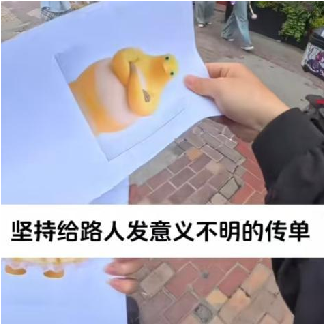
\includegraphics[width=132.74bp,height=0.76\textheight,keepaspectratio]{figures/chapter03/figure03_2.pdf}
  \renewcommand{\thefigure}{3.2}
  \caption{奶蛙的图片被大量用作意义不明传单挑战}
  \label{fig:03-2}
\end{figure}


然而，目前的奶蛙仅仅是奶龙的附庸，缺少自己的独到特色。

而最好的特色，无疑就是一个充满魔性的声音。


\clearpage
% !TEX root = ../main.tex

\clearpage
% Source PDF page 8.
\section{第四章\quad 奶蛙捧腹大笑的诞生与发展史}

主播王麻衣在直播的时候，有一个叫做布洛芬的青年用户连麦。连麦之后，青年不知为何一直发出异常爽朗的大笑声，把所有人都搞破绷了。~(见\figref{fig:04-1})

音效与形象的联姻意义重大\textsuperscript{[1]}。如同黑雷霆目力咆哮与野兽先辈一个一个一个表情的搭配一样，这经典的笑声便流传下来，成为了奶蛙捧腹大笑的灵魂音色。

% !TEX root = ../../main.tex
\begin{figure}[H]
  \centering
  
\includegraphics[width=147.02bp,height=0.76\textheight,keepaspectratio]{figures/chapter04/figure04_1.pdf}
  \renewcommand{\thefigure}{4.1}
  \caption{听到奶蛙大笑原声而震惊不已的主播}
  \label{fig:04-1}
\end{figure}


而结合 AI 视频生成，我们现在所熟知的奶蛙形象便出现在我们的面前！~(见\figref{fig:04-2})

% !TEX root = ../../main.tex
\begin{figure}[H]
  \centering
  
\includegraphics[width=160bp,height=0.76\textheight,keepaspectratio]{figures/chapter04/figure04_2.pdf}
  \renewcommand{\thefigure}{4.2}
  \caption{完全胜利！奶蛙最经典的捧腹大笑形象}
  \label{fig:04-2}
\end{figure}


奶蛙们捧腹大笑的时候，大家会在弹幕上刷“众宾欢也”、“齐齐哈尔”。这种现代网络翻译梗无疑为奶家人们空耳、联想等创造力的激发注入了活力。

2026 年 3 月，奶龙官方呼吁停止丑化二创，关闭视频评论区并批量拉黑发布奶蛙的账号。

但是奶蛙的影响力已经扩散开来（潘多拉奶盒打开了），难以制止了。

至此，奶蛙凭借着魔性而意义不明的捧腹大笑，正式脱离了奶龙，成为了互联网上一个强而有力的热梗。

\clearpage
% Source PDF page 9.
% !TEX root = ../../main.tex
\clearpage
\begin{figure}[H]
  \centering
  \phantomsection
  \addcontentsline{lof}{figure}{\protect\numberline{}2026 年 10 月 2 日，奶蛙迎来 2 岁生日}
  
\includegraphics[width=339.39bp,height=0.90\textheight,keepaspectratio]{figures/chapter04/birthdayPlate.pdf}
  \caption*{2026 年 10 月 2 日，奶蛙迎来 2 岁生日}
\end{figure}

\clearpage



\clearpage
% !TEX root = ../main.tex

\clearpage
% Source PDF page 10.
\section{第五章\quad 捧腹大笑思想理论体系}

捧腹大笑对年轻人有什么魔力？关于这个问题，我们可以通过深入的思考，建立奶蛙捧腹大笑思想理论体系（迫真）。~(见\figref{fig:05-1})

% !TEX root = ../../main.tex
\begin{figure}[H]
  \centering
  
\includegraphics[width=127.74bp,height=0.76\textheight,keepaspectratio]{figures/chapter05/figure05_1.pdf}
  \renewcommand{\thefigure}{5.1}
  \caption{奶蛙的城府.jpg}
  \label{fig:05-1}
\end{figure}


\subsection{一、情绪代偿：把“绷不住”合法化}

考研、绩点、就业的复合压力下，负面情绪缺少体面的出口。奶蛙提供了一种\textquotedbl{}笑着崩溃\textquotedbl{}的姿态——既表达了失控，又不至于沉重。~(见\figref{fig:05-2})

% !TEX root = ../../main.tex
\begin{figure}[H]
  \centering
  
\includegraphics[width=128.76bp,height=0.76\textheight,keepaspectratio]{figures/chapter05/figure05_2.pdf}
  \renewcommand{\thefigure}{5.2}
  \caption{奶蛙的请假条}
  \label{fig:05-2}
\end{figure}


\subsection{二、群体稀释：用“我们”消解“我”}

用一张梗图代替自述，把“我很差劲”翻译成“我们都这样”。个体暴露被群体化收编，自嘲因而不必付出羞耻成本。~(见\figref{fig:05-3})

% !TEX root = ../../main.tex
\begin{figure}[H]
  \centering
  
\includegraphics[width=109.89bp,height=0.76\textheight,keepaspectratio]{figures/chapter05/figure05_3.pdf}
  \renewcommand{\thefigure}{5.3}
  \caption{大家都在大笑，就不显得我糖了}
  \label{fig:05-3}
\end{figure}


\clearpage
% Source PDF page 11.
\subsection{三、反精致：对优秀人设的审美罢工}

大学生被期待为“精致的、上进的、有规划的人”。转发一只丑、怪、抽象的奶蛙，是一次低成本的不合作表态。~(见\figref{fig:05-4})

% !TEX root = ../../main.tex
\begin{figure}[H]
  \centering
  
\includegraphics[width=143.14bp,height=0.76\textheight,keepaspectratio]{figures/chapter05/figure05_4.pdf}
  \renewcommand{\thefigure}{5.4}
  \caption{做题龙...？}
  \label{fig:05-4}
\end{figure}


\subsection{四、学校社交：人的本质是复读机}

集体居住让奶蛙拥有“线上”“面对面”双通道传播途径。同一个梗在同一屋檐下被反复复诵，趣味衰减极慢。~(见\figref{fig:05-5})

% !TEX root = ../../main.tex
\begin{figure}[H]
  \centering
  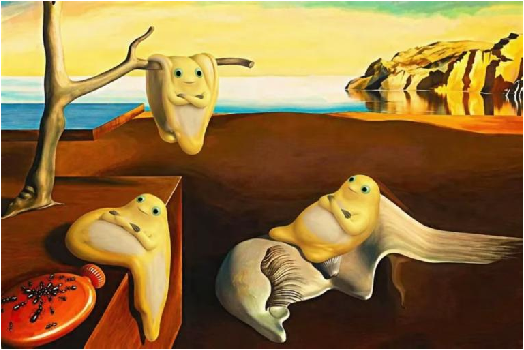
\includegraphics[width=213.93bp,height=0.76\textheight,keepaspectratio]{figures/chapter05/figure05_5.pdf}
  \renewcommand{\thefigure}{5.5}
  \caption{世界名画：永恒的奶蛙}
  \label{fig:05-5}
\end{figure}


\subsection{五、逆反认证：官方压制变成亚文化勋章}

2026 年 3 月，奶龙官方关评、拉黑，反而被网友读作“官方破防”。权威的否认，成了 meme 含金量的最高背书，热度此后一发不可收拾。~(见\figref{fig:05-6})

% !TEX root = ../../main.tex
\begin{figure}[H]
  \centering
  
\includegraphics[width=107.64bp,height=0.76\textheight,keepaspectratio]{figures/chapter05/figure05_6.pdf}
  \renewcommand{\thefigure}{5.6}
  \caption{喂，你打压奶蛙打压的很开心啊（全恼）}
  \label{fig:05-6}
\end{figure}


（不行，扯不下去了）

奶蛙：五重战神，出来！

如此的大笑魔神，又有谁能挡？！TM 的有谁能挡了？！


\clearpage
% !TEX root = ../main.tex

\clearpage
% Source PDF page 12.
\section{第六章\quad 奶蛙的衍生语与衍生动作}

奶蛙产生了许多奇妙的衍生语（绝大多数来源于王者荣耀中不知火舞语音的变速变调）和衍生动作。我们将会一一说明并提及有关的著名奶蛙二创作品。

\subsection{一、衍生语——安迪}

主要运用场景为爬行奶龙说话效果、奶蛋说话效果、奶蛙出场说话效果等，奶蛙高频说话效果之一。等效空耳有“俺滴”“安定”“俺无敌”“暗地”等。

\subsection{二、衍生语——嘎嘎滴辣虾}

运用场景广泛，奶蛙高频说话效果之一。等效空耳为“刚刚点了谁”“刚刚跌落水”“刚刚掉了什”等。

\subsection{三、衍生语——卡脚先}

主要运用场景为奶蛙小剧场的转折或收尾。等效空耳为“刚救下”“赶紧写”“干啥先”“啃脚先”等。

\subsection{四、衍生语——无了}

主要运用场景为奶蛙吃瘪、惊讶音效。等效空耳为“哦了”“好了”等。~(见\figref{fig:06-1})

% !TEX root = ../../main.tex
\begin{figure}[H]
  \centering
  
\includegraphics[width=128bp,height=0.76\textheight,keepaspectratio]{figures/chapter06/figure06_1.pdf}
  \renewcommand{\thefigure}{6.1}
  \caption{常伴随无了的奶蛙抱头动作}
  \label{fig:06-1}
\end{figure}


\subsection{五、衍生语——甘巴爹}

主要运用场景为奶蛙肯定、疑问音效。等效空耳为“干扒地”“刚拔的”等。

\subsection[六、衍生语——有用不]{六、衍生语——有用不~(见\figref{fig:06-2})}

主要用途为丰富奶蛙的语言，一般作为安迪的下位替代。等效空耳为“忧郁菇”“犹豫不”等。

% !TEX root = ../../main.tex
\begin{figure}[H]
  \centering
  
\includegraphics[width=55bp]{figures/chapter06/figure06_2.png}
  \renewcommand{\thefigure}{6.2}
  \caption{有用不？}
  \label{fig:06-2}
\end{figure}


\subsection[七、衍生动作——思考与抱胸]{七、衍生动作——思考与抱胸~(见\figref{fig:06-3})}

% !TEX root = ../../main.tex
\begin{figure}[H]
  \centering
  
\includegraphics[width=84.8bp,height=0.76\textheight,keepaspectratio]{figures/chapter06/figure06_3.pdf}
  \renewcommand{\thefigure}{6.3}
  \caption{蹲起大笑的奶蛙}
  \label{fig:06-3}
\end{figure}


\clearpage
\subsection{八、衍生动作——蹲起大笑}

% !TEX root = ../../main.tex
\begin{figure}[H]
  \centering
  
\includegraphics[height=70bp]{figures/chapter06/figure06_4.pdf}\qquad
  
\includegraphics[height=70bp]{figures/chapter06/seasideLaughter.png}
  \renewcommand{\thefigure}{6.4}
  \caption{单人蹲起大笑（左）与海边双人大笑（右）}
  \label{fig:06-4}
\end{figure}


% Source PDF page 13.
熟悉蹲起大笑的人肯定知道，蹲起大笑还有双人组合技甚至多人组合技——因为画面过于神圣和有伤风化，我们按下不表（你只是怕了）。~(见\figref{fig:06-4})

\subsection{九、衍生动作——爬行}

% !TEX root = ../../main.tex
\begin{figure}[H]
  \centering
  
\includegraphics[width=111.32bp,height=0.76\textheight,keepaspectratio]{figures/chapter06/figure06_5.pdf}
  \renewcommand{\thefigure}{6.5}
  \caption{正在爬行前进的奶蛙}
  \label{fig:06-5}
\end{figure}


爬行奶蛙在爬到一半时会看向屏幕，说出一声“安迪”，然后继续爬行。~(见\figref{fig:06-5})

\subsection{十、衍生动作——摆架势}

% !TEX root = ../../main.tex
\begin{figure}[H]
  \centering
  
\includegraphics[width=92.55bp,height=0.76\textheight,keepaspectratio]{figures/chapter06/figure06_6.pdf}
  \renewcommand{\thefigure}{6.6}
  \caption{和读者对视的奶蛙}
  \label{fig:06-6}
\end{figure}


奶蛙的招牌动作之一。模仿奶蛙的青年们最常摆这个动作。~(见\figref{fig:06-6})

\clearpage
\subsection{十一、衍生动作——对视}

% !TEX root = ../../main.tex
\begin{figure}[H]
  \centering
  
\includegraphics[width=93.77bp,height=0.76\textheight,keepaspectratio]{figures/chapter06/figure06_7.pdf}
  \renewcommand{\thefigure}{6.7}
  \caption{正在打坐的奶蛙}
  \label{fig:06-7}
\end{figure}


谁说奶蛙不是福瑞？奶蛙作为动物，很好的融入了“有两个福瑞在对视”的梗图，并且难绷程度青出于蓝。~(见\figref{fig:06-7})

\subsection[十二、衍生动作——打坐]{十二、衍生动作——打坐~(见\figref{fig:06-8})}

% !TEX root = ../../main.tex
\begin{figure}[H]
  \centering
  
\includegraphics[width=85.31bp,height=0.76\textheight,keepaspectratio]{figures/chapter06/figure06_8.pdf}
  \renewcommand{\thefigure}{6.8}
  \caption{正在魅惑读者的奶蛙}
  \label{fig:06-8}
\end{figure}


% Source PDF page 14.
\subsection[十三、衍生动作——魅惑]{十三、衍生动作——魅惑~(见\figref{fig:06-9})}

% !TEX root = ../../main.tex
\begin{figure}[H]
  \centering
  
\includegraphics[width=103.67bp,height=0.76\textheight,keepaspectratio]{figures/chapter06/figure06_9.pdf}
  \renewcommand{\thefigure}{6.9}
  \caption{低头握拳的奶蛙}
  \label{fig:06-9}
\end{figure}


\clearpage
\subsection[十四、衍生动作——低头握拳]{十四、衍生动作——低头握拳~(见\figref{fig:06-10})}

% !TEX root = ../../main.tex
\begin{figure}[H]
  \centering
  
\includegraphics[width=103.67bp,height=0.76\textheight,keepaspectratio]{figures/chapter06/figure06_10.pdf}
  \renewcommand{\thefigure}{6.10}
  \caption{低头握拳的奶蛙}
  \label{fig:06-10}
\end{figure}


\subsection[十五、衍生动作——啃脚]{十五、衍生动作——啃脚~(见\figref{fig:06-11})}

% !TEX root = ../../main.tex
\begin{figure}[H]
  \centering
  
\includegraphics[width=91.22bp,height=0.76\textheight,keepaspectratio]{figures/chapter06/figure06_11.pdf}
  \renewcommand{\thefigure}{6.11}
  \caption{正在低头啃脚的奶蛙}
  \label{fig:06-11}
\end{figure}


\subsection[十六、衍生动作——连续放屁]{十六、衍生动作——连续放屁~(见\figref{fig:06-12})}

% !TEX root = ../../main.tex
\begin{figure}[H]
  \centering
  
\includegraphics[width=114.58bp,height=0.76\textheight,keepaspectratio]{figures/chapter06/figure06_12.pdf}
  \renewcommand{\thefigure}{6.12}
  \caption{正在发动沼气动力的奶蛙}
  \label{fig:06-12}
\end{figure}


奶蛙的招牌雷霆动图动作之一。放屁的奶蛙会左右开弓连续释放气体，最后以一发蓄力的巨响收尾。

\clearpage
% !TEX root = ../main.tex

\clearpage
% Source PDF page 15.
\section{第七章\quad 人工智能对变种奶蛙生产传播的广泛推动}

由于人工智能的迅猛发展，人工智能的生图能力和视频生成能力水涨船高。于是，本就抽象无比的奶蛙，在 AI 的助推下变得更加神圣。

\subsection{一、换皮奶蛙}

换皮奶蛙指的是仅皮肤发生变化，大部分形体特征保留下来的变种奶蛙。

\subsubsection[（1）异色奶蛙]{（1）异色奶蛙~(见\figref{fig:07-1})}

% !TEX root = ../../main.tex
\begin{figure}[H]
  \centering
  
\includegraphics[width=203.32bp,height=0.76\textheight,keepaspectratio]{figures/chapter07/figure07_1.pdf}
  \renewcommand{\thefigure}{7.1}
  \caption{一些不同模式的异色奶蛙形象}
  \label{fig:07-1}
\end{figure}


\subsubsection{（2）植奶、僵奶}

B 站 up 主暖气杀手 AAA 所制作的《植奶大战僵龙》系列，无疑是奶蛙爆火的强力引擎之一。其通过将奶蛙和 PVZ 结合，成功做出多款百万播放视频。~(见\figref{fig:07-2})

% !TEX root = ../../main.tex
\begin{figure}[H]
  \centering
  
\includegraphics[width=272.48bp,height=0.76\textheight,keepaspectratio]{figures/chapter07/figure07_2.pdf}
  \renewcommand{\thefigure}{7.2}
  \caption{《植奶大战僵龙》系列视频中的海豚僵奶和猫尾奶形象}
  \label{fig:07-2}
\end{figure}


\subsubsection{（3）其他}

其他大部分换皮奶蛙都是用图标、封面等进行换皮，举例如下。~(见\figref{fig:07-3})

\clearpage
% Source PDF page 16.
% !TEX root = ../../main.tex
\begin{figure}[H]
  \centering
  
\includegraphics[width=280.02bp,height=0.76\textheight,keepaspectratio]{figures/chapter07/figure07_3.pdf}
  \renewcommand{\thefigure}{7.3}
  \caption{线代课本奶蛙（左） VIVO 奶蛙（中） 学习通奶蛙（右）}
  \label{fig:07-3}
\end{figure}


\subsection{二、异形奶蛙}

异形奶蛙指的是丢失大量形体特征，但是仍然保留眼睛和大笑的变种奶蛙。

\subsubsection{（1）奶蛋}

% !TEX root = ../../main.tex
\begin{figure}[H]
  \centering
  
\includegraphics[width=104.28bp,height=0.76\textheight,keepaspectratio]{figures/chapter07/figure07_4.pdf}
  \renewcommand{\thefigure}{7.4}
  \caption{奶蛋的形象}
  \label{fig:07-4}
\end{figure}


\textbf{奶蛋（Milk Egg）}，将奶蛙简化到极致的产物。~(见\figref{fig:07-4})

在 B 站 up 主奶史\_所制作的《选择你的奶伴》系列视频中高频出现，与衍生语“安迪”高频结伴出现，几乎从无败绩。因此产生了“奶蛋轮椅”的说法，把“安迪”等价空耳为“俺无敌”。

现在奶蛋已经默认为奶伴中的至强者之一，\textbf{拥有强大的运气和极为逆天的能力}（包括但不限于空间转移/转变、时间加速、召唤陨石、催眠洗脑）。“安迪”一出，谁与争锋。但在一些日常向作品中，奶蛋不会表现出其实力。

\subsubsection[（2）奶狗\&奶屎、奶鸡、奶鼠\&奶粉、奶茶、豆奶等]{（2）奶狗\&奶屎、奶鸡、奶鼠\&奶粉、奶茶、豆奶等~(见\figref{fig:07-5})}

% !TEX root = ../../main.tex
\begin{figure}[H]
  \centering
  
\includegraphics[width=199.14bp,height=0.76\textheight,keepaspectratio]{figures/chapter07/figure07_5.pdf}
  \renewcommand{\thefigure}{7.5}
  \caption{奶狗（左）和奶屎（右）的形象}
  \label{fig:07-5}
\end{figure}


\textbf{奶狗（Milk Dog）}由于其蠢萌的形象，从十二奶肖中脱颖而出。智商较低，有敏锐的嗅觉，拥有特有动作打滚转圈大笑。

值得注意的是，单只奶狗的能力虽然非常弱，但是一群奶狗的能力将得到显著提升。在奶狗极度愤怒并且拥有项链的情况下，其能够使用召唤术召唤数只小奶狗为自己作战，两只小奶狗合作的威力就能够接近于奶蛙。

\clearpage
% Source PDF page 17.
在某些情况下，奶狗能够使用嗅觉寻找奶蛋，来短暂获得奶蛋的无敌能力。~(见\figref{fig:07-6})

% !TEX root = ../../main.tex
\begin{figure}[H]
  \centering
  
\includegraphics[width=237.8bp,height=0.76\textheight,keepaspectratio]{figures/chapter07/figure07_6.pdf}
  \renewcommand{\thefigure}{7.6}
  \caption{召唤出四只小奶狗的奶狗}
  \label{fig:07-6}
\end{figure}


\textbf{奶屎（Milk Shit）}是与奶狗绑定的形象。可以由奶狗的体内排出，具有吸引奶狗的能力（毕竟狗改不了吃奥利给嘛）。一般没有移动能力，会对身边的奶伴大笑。但在一些作品中，可以长出小短腿进行缓慢的移动。

% !TEX root = ../../main.tex
\begin{figure}[H]
  \centering
  
\includegraphics[width=177.31bp,height=0.76\textheight,keepaspectratio]{figures/chapter07/figure07_7.pdf}
  \renewcommand{\thefigure}{7.7}
  \caption{奶鼠（左）和奶粉（右）的形象}
  \label{fig:07-7}
\end{figure}


\textbf{奶鸡（Milk Hen）}从十二奶肖中脱颖而出的原因并不是造型，而是和奶蛋有着现实逻辑的强相关性。奶鸡具有一定的滑翔和缓降能力，可以进行奶蛋的生产。~(见\figref{fig:07-7})

% !TEX root = ../../main.tex
\begin{figure}[H]
  \centering
  
\includegraphics[width=111.93bp,height=0.76\textheight,keepaspectratio]{figures/chapter07/figure07_8.pdf}
  \renewcommand{\thefigure}{7.8}
  \caption{奶茶的形象}
  \label{fig:07-8}
\end{figure}


\textbf{奶鼠（Milk Rat）}由于其可爱萌趣的形象，从十二奶肖中脱颖而出。情商较低，常常因为做嘲讽动作而被远程攻击手段弄翻车，拥有特有语音“奶鼠奶鼠”。~(见\figref{fig:07-8})

\textbf{奶粉（Pink Naiwa）}是与奶鼠绑定的形象。除了身体颜色外，没有与正常奶蛙的明显区别，一般认为其是奶蛙族的雌性个体。其拥有\textbf{必定能全方位克制奶鼠并一定使其吃瘪的能力}（人称“奶鼠最严厉的母亲”）。

\clearpage
% Source PDF page 18.

% !TEX root = ../../main.tex
\begin{figure}[H]
  \centering
  
\includegraphics[width=111.93bp,height=0.76\textheight,keepaspectratio]{figures/chapter07/figure07_9.pdf}
  \renewcommand{\thefigure}{7.9}
  \caption{奶茶的形象}
  \label{fig:07-9}
\end{figure}


\textbf{奶茶（Milk Teacup）}常常作为饮品以复数形式出现。和奶蛋的关系貌似很好。~(见\figref{fig:07-9})

% !TEX root = ../../main.tex
\begin{figure}[H]
  \centering
  
\includegraphics[width=176.8bp,height=0.76\textheight,keepaspectratio]{figures/chapter07/figure07_10.pdf}
  \renewcommand{\thefigure}{7.10}
  \caption{豆奶的原型（左）和经典形象（右）}
  \label{fig:07-10}
\end{figure}


\textbf{豆奶（Nai Doubao）}，豆包和奶蛙的结合体。由于豆包被大家默认为能上桌的 AI 中的最弱档次，于是就和奶龙糖糖联合，形成了豆奶的前身。在奶蛙热度飙升之后，豆包和奶蛙结合形成了豆奶。拥有豆包特有的大笑声音。~(见\figref{fig:07-10})

以上经典形象及其性格特点多在 B 站 up 主奶史\_所制作的《选择你的奶伴》系列中成功深入人心，为奶蛙世界观奠定了根本性的基础。

\subsubsection{（3）奶蛙娘}

% !TEX root = ../../main.tex
\begin{figure}[H]
  \centering
  
\includegraphics[width=188.63bp,height=0.76\textheight,keepaspectratio]{figures/chapter07/figure07_11.pdf}
  \renewcommand{\thefigure}{7.11}
  \caption{“最绝的角色设计”}
  \label{fig:07-11}
\end{figure}


奶蛙最经典的娘化形象之一（搜不到原画师 qwq）。~(见\figref{fig:07-11})

由于奶蛙的手是黑色的，奶蛙娘的手也是黑色的。由此产生了一个有趣的关联梗：在游戏《魔法少女的魔女审判》中，魔女化的魔法少女的手也会变黑。因此，可以把奶蛙看作奶蛙娘魔奶化后的残骸。~(见\figref{fig:07-12})

\clearpage
% Source PDF page 19.
% !TEX root = ../../main.tex
\begin{figure}[H]
  \centering
  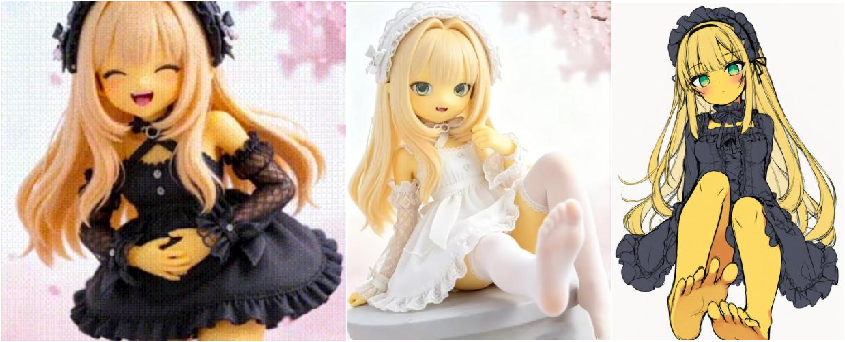
\includegraphics[width=188.63bp,height=0.76\textheight,keepaspectratio]{figures/chapter07/figure07_12.pdf}
  \renewcommand{\thefigure}{7.12}
  \caption{“最绝的角色设计”}
  \label{fig:07-12}
\end{figure}


\subsubsection{（4）奶蝠}

% !TEX root = ../../main.tex
\begin{figure}[H]
  \centering
  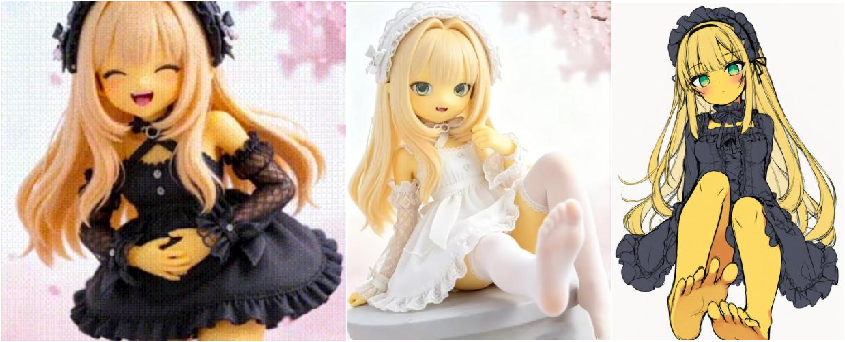
\includegraphics[width=129.88bp,height=0.76\textheight,keepaspectratio]{figures/chapter07/figure07_13.pdf}
  \renewcommand{\thefigure}{7.13}
  \caption{奶正太的形象}
  \label{fig:07-13}
\end{figure}


奶蛙最经典的娘化形象之一，二创最多最神的娘化奶蛙形象。辣眼本《奶莉的诞生》和辣眼 galgame《见习的幸福天使：奶福》采用的就是奶蝠的形象。~(见\figref{fig:07-13})

奶蝠一般以黑色洛丽塔少女的模样出现，本体是一只吸血鬼奶蛙。奶蝠的本体（即吸血鬼奶蛙）具有黑色的巨型翅膀、尖锐的牙齿和又长又尖的耳朵，具有一定的飞行能力。我们姑且认为奶蝠不会随着外貌的变化改变性别。

\subsubsection{（5）奶正太}

% !TEX root = ../../main.tex
\begin{figure}[H]
  \centering
  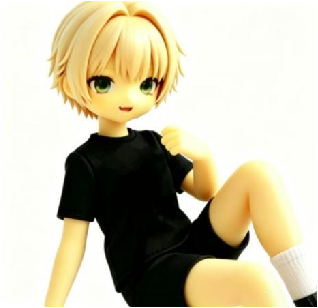
\includegraphics[width=308.28bp,height=0.76\textheight,keepaspectratio]{figures/chapter07/figure07_14.pdf}
  \renewcommand{\thefigure}{7.14}
  \caption{奶龙娘的形象}
  \label{fig:07-14}
\end{figure}


奶蛙的正太形象，和奶蝠的定位类似。~(见\figref{fig:07-14})

\clearpage
% Source PDF page 20.
\subsubsection{（6）奶龙娘}

% !TEX root = ../../main.tex
\begin{figure}[H]
  \centering
  
\includegraphics[width=308.28bp,height=0.76\textheight,keepaspectratio]{figures/chapter07/figure07_15.pdf}
  \renewcommand{\thefigure}{7.15}
  \caption{奶龙娘的形象}
  \label{fig:07-15}
\end{figure}


更偏向奶龙的经典娘化形象之一。~(见\figref{fig:07-15})

\subsubsection{（7）奶蛙妹}

% !TEX root = ../../main.tex
\begin{figure}[H]
  \centering
  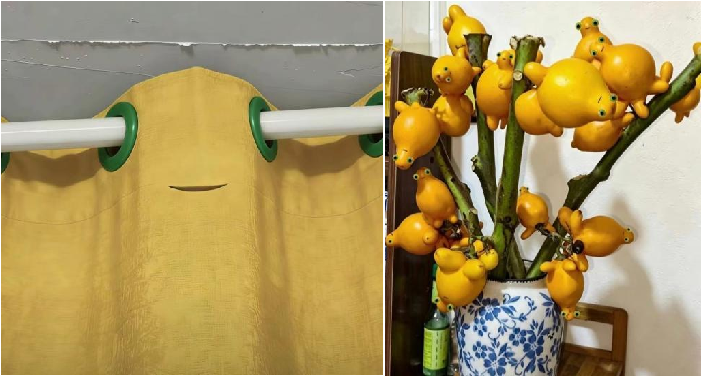
\includegraphics[width=286.45bp,height=0.76\textheight,keepaspectratio]{figures/chapter07/figure07_16.pdf}
  \renewcommand{\thefigure}{7.16}
  \caption{生活中的奶帘（左）和奶五味子盆景（右）}
  \label{fig:07-16}
\end{figure}


画风备受好评的新生代奶蛙娘化形象。作者为 ality5s（小红书）。~(见\figref{fig:07-16})

\subsubsection{（8）西格玛奶蛙}

% !TEX root = ../../main.tex
\begin{figure}[H]
  \centering
  
\includegraphics[width=128.86bp,height=0.76\textheight,keepaspectratio]{figures/chapter07/figure07_17.pdf}
  \renewcommand{\thefigure}{7.17}
  \caption{正在捧腹大笑的 deepseek 鲸鱼}
  \label{fig:07-17}
\end{figure}


奶蛙的硬汉形象，西格玛效果套用在奶蛙身上的产物。~(见\figref{fig:07-17})

\clearpage
% Source PDF page 21.
\subsubsection{（9）现实幻视}

生活中和奶蛙形象神似的物品，较为稀有。~(见\figref{fig:07-18})

% !TEX root = ../../main.tex
\begin{figure}[H]
  \centering
  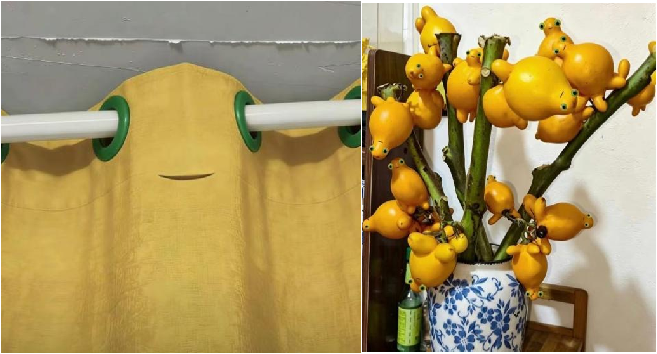
\includegraphics[width=268.09bp,height=0.76\textheight,keepaspectratio]{figures/chapter07/figure07_18.pdf}
  \renewcommand{\thefigure}{7.18}
  \caption{生活中的奶帘（左）和奶五味子盆景（右）}
  \label{fig:07-18}
\end{figure}


\subsubsection{（10）其他 AI 的奶化形象}

作为奶蛙的助推者，除了豆包形成的豆奶外，其他 AI 也受到了奶化。我们在这里以 deepseek、OpenAI、Anthropic、Grok 等为典型代表进行展示。~(见\figref{fig:07-19}, \figref{fig:07-20}, \figref{fig:07-21}, \figref{fig:07-22})

% !TEX root = ../../main.tex
\begin{figure}[H]
  \centering
  
\includegraphics[width=232.59bp,height=0.76\textheight,keepaspectratio]{figures/chapter07/figure07_19.pdf}
  \renewcommand{\thefigure}{7.19}
  \caption{“奶蛋神力由来的传说”}
  \label{fig:07-19}
\end{figure}


% !TEX root = ../../main.tex
\begin{figure}[H]
  \centering
  
\includegraphics[width=229.53bp,height=0.76\textheight,keepaspectratio]{figures/chapter07/figure07_20.pdf}
  \renewcommand{\thefigure}{7.20}
  \caption{奶工智能四巨头}
  \label{fig:07-20}
\end{figure}


% !TEX root = ../../main.tex
\begin{figure}[H]
  \centering
  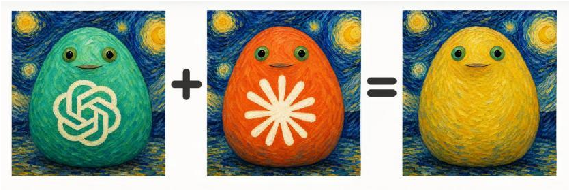
\includegraphics[width=251.97bp,height=0.76\textheight,keepaspectratio]{figures/chapter07/figure07_21.pdf}
  \renewcommand{\thefigure}{7.21}
  \caption{奶菜的形象（左）和奶葡的形象（右）}
  \label{fig:07-21}
\end{figure}


\clearpage
% Source PDF page 22.
% !TEX root = ../../main.tex
\begin{figure}[H]
  \centering
  
\includegraphics[width=116.72bp,height=0.76\textheight,keepaspectratio]{figures/chapter07/figure07_22.pdf}
  \renewcommand{\thefigure}{7.22}
  \caption{伪装成美团袋鼠的奶蛙}
  \label{fig:07-22}
\end{figure}


\subsubsection{（11）其他}

主要为生活中物品奶龙化的样子。由于篇幅原因，仅在这里举两例。~(见\figref{fig:07-23})

% !TEX root = ../../main.tex
\begin{figure}[H]
  \centering
  
\includegraphics[width=251.97bp,height=0.76\textheight,keepaspectratio]{figures/chapter07/figure07_23.pdf}
  \renewcommand{\thefigure}{7.23}
  \caption{奶菜的形象（左）和奶葡的形象（右）}
  \label{fig:07-23}
\end{figure}


\subsection{三、主要客串角色}

\subsubsection{（1）美团袋鼠}

因为肥嘟嘟的颜色与奶蛙相近，常常与奶蛙联动出场。~(见\figref{fig:07-24})

% !TEX root = ../../main.tex
\begin{figure}[H]
  \centering
  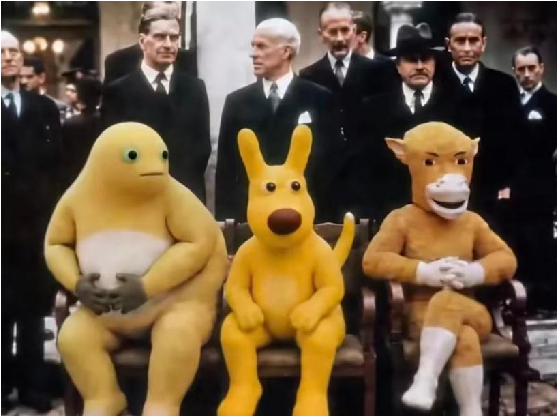
\includegraphics[width=116.72bp,height=0.76\textheight,keepaspectratio]{figures/chapter07/figure07_24.pdf}
  \renewcommand{\thefigure}{7.24}
  \caption{伪装成美团袋鼠的奶蛙}
  \label{fig:07-24}
\end{figure}


\clearpage
% Source PDF page 23.
\subsubsection{（2）牛来、牛来妈}

因为牛来妈的颜色与奶蛙相近，而且牛来和奶蛙抽象程度平分秋色，因此两母子和奶蛙也常常联动出场。~(见\figref{fig:07-25}, \figref{fig:07-26})

% !TEX root = ../../main.tex
\begin{figure}[H]
  \centering
  
\includegraphics[width=246.36bp,height=0.76\textheight,keepaspectratio]{figures/chapter07/figure07_25.pdf}
  \renewcommand{\thefigure}{7.25}
  \caption{伪装成牛来妈的奶蛙（左）和捧腹大笑的牛来（右）}
  \label{fig:07-25}
\end{figure}


% !TEX root = ../../main.tex
\begin{figure}[H]
  \centering
  
\includegraphics[width=227.8bp,height=0.76\textheight,keepaspectratio]{figures/chapter07/figure07_26.pdf}
  \renewcommand{\thefigure}{7.26}
  \caption{恶搞历史照片：雅尔糖会议三巨头}
  \label{fig:07-26}
\end{figure}


\subsubsection{（3）熊大、熊二}

因为熊二颜色与奶蛙相近，而且熊大有“轻松绷住”、“绷不住了”的梗和奶蛙大笑高度契合，因此两兄弟和奶蛙有时也会联动出场，次数较少。~(见\figref{fig:07-27})

% !TEX root = ../../main.tex
\begin{figure}[H]
  \centering
  
\includegraphics[width=102.85bp,height=0.76\textheight,keepaspectratio]{figures/chapter07/figure07_27.pdf}
  \renewcommand{\thefigure}{7.27}
  \caption{捧腹大笑的蕾雅}
  \label{fig:07-27}
\end{figure}


\clearpage
% Source PDF page 24.
\subsubsection{（4）水豚噜噜}

因为噜噜颜色与奶蛙相近，因此和奶蛙有时也会联动出场，次数较少。~(见\figref{fig:07-28})

% !TEX root = ../../main.tex
\begin{figure}[H]
  \centering
  
\includegraphics[width=90.41bp,height=0.76\textheight,keepaspectratio]{figures/chapter07/figure07_28.pdf}
  \renewcommand{\thefigure}{7.28}
  \caption{今天，仁者安迪就要捧他的最后一腹！}
  \label{fig:07-28}
\end{figure}


\subsubsection{（5）说的道理}

由于电棍发出的的神秘动静，说的道理拥有多种唐笑，而且作为动物园的一代抽象宗师，道理经常夺舍其他人，绝对有资格驾驭奶蛙的力量。

道理究竟有几种形态呢？~(见\figref{fig:07-29})

% !TEX root = ../../main.tex
\begin{figure}[H]
  \centering
  
\includegraphics[width=138.45bp,height=0.76\textheight,keepaspectratio]{figures/chapter07/figure07_29.pdf}
  \renewcommand{\thefigure}{7.29}
  \caption{道理奶蛙}
  \label{fig:07-29}
\end{figure}


\subsubsection{（6）绿猪}

愤怒的小鸟中的主要敌人。由于其在玩家失败时的嘲讽笑容过于魔性，形成了一套使用频率较高的绿猪笑笑表情包。而既然绿猪以笑出圈，就自然而然地和奶蛙强强联合，形成了奶蛙的绿猪模式。~(见\figref{fig:07-30})

% !TEX root = ../../main.tex
\begin{figure}[H]
  \centering
  
\includegraphics[width=133.25bp,height=0.76\textheight,keepaspectratio]{figures/chapter07/figure07_30.pdf}
  \renewcommand{\thefigure}{7.30}
  \caption{绿猪奶蛙}
  \label{fig:07-30}
\end{figure}


\clearpage
% Source PDF page 25.

\subsection{四、次要客串角色}

次要客串角色的定义是：在一定的圈子内拥有奶之名号，但是并没有像主要客串角色那样破圈被大量使用于表情包传播、二创制作的角色。

\subsubsection{（1）莲见蕾雅}

莲见蕾雅，视觉小说游戏《魔法少女的魔女审判》中 13 名囚犯少女之一。在游戏二周目中，蕾雅成为了二周目希罗小团体的成员，角色定位类似于一周目艾玛小团体的橘雪莉，结果直接从冷静优雅的明星演员滑坡成了一直糖笑的嘉豪逗比（名场面“嘿嘿，哈哈哈哈\textasciitilde{}”），又是金毛，因此被称为魔裁奶龙。

13 名囚犯少女之一的远野汉娜形象要素更接近奶蛙一点（金发而且眼睛也是绿色的），但她的性格一点不像奶蛙。而明明蕾雅眼睛并不是绿色的，却能凭借堪比奶蛙的糖度脱颖而出，这启示我们：只要糖分够，即使没有奶蛙的外表，也拥有了奶蛙的灵魂。

由于名字里有个“蕾”字，蕾雅还和蕾忍宗有着紧密的联系（握握手握握双手），我们在这里按下不表。~(见\figref{fig:07-31})

% !TEX root = ../../main.tex
\begin{figure}[H]
  \centering
  
\includegraphics[width=215.05bp,height=0.76\textheight,keepaspectratio]{figures/chapter07/figure07_31.pdf}
  \renewcommand{\thefigure}{7.31}
  \caption{一周目被串串香的蕾雅（左）和二周目捧腹大笑的蕾雅（右）}
  \label{fig:07-31}
\end{figure}


\subsubsection{（2）刹暗天}

刹暗天，港漫《武神》中的中后期主角、港漫《武神终极》中实力最强的终极强者之一（《海虎》三部曲中最强者白首男转世）。以摸鱼摆烂的性格而出名。因为其五级命格“仁者暗帝”可以被空耳为“仁者安迪”，招式暗天车轮拳可以看成奶蛙拳，莫名其妙就和奶蛙扯上了关系。~(见\figref{fig:07-32})

% !TEX root = ../../main.tex
\begin{figure}[H]
  \centering
  
\includegraphics[width=90.41bp,height=0.76\textheight,keepaspectratio]{figures/chapter07/figure07_32.pdf}
  \renewcommand{\thefigure}{7.32}
  \caption{今天，仁者安迪就要捧他的最后一腹！}
  \label{fig:07-32}
\end{figure}


\clearpage
% Source PDF page 26.
% !TEX root = ../../main.tex
\clearpage
\begin{figure}[H]
  \centering
  \phantomsection
  \addcontentsline{lof}{figure}{\protect\numberline{}奶蝠的真身——美丽诱惑下的奶之恶魔}
  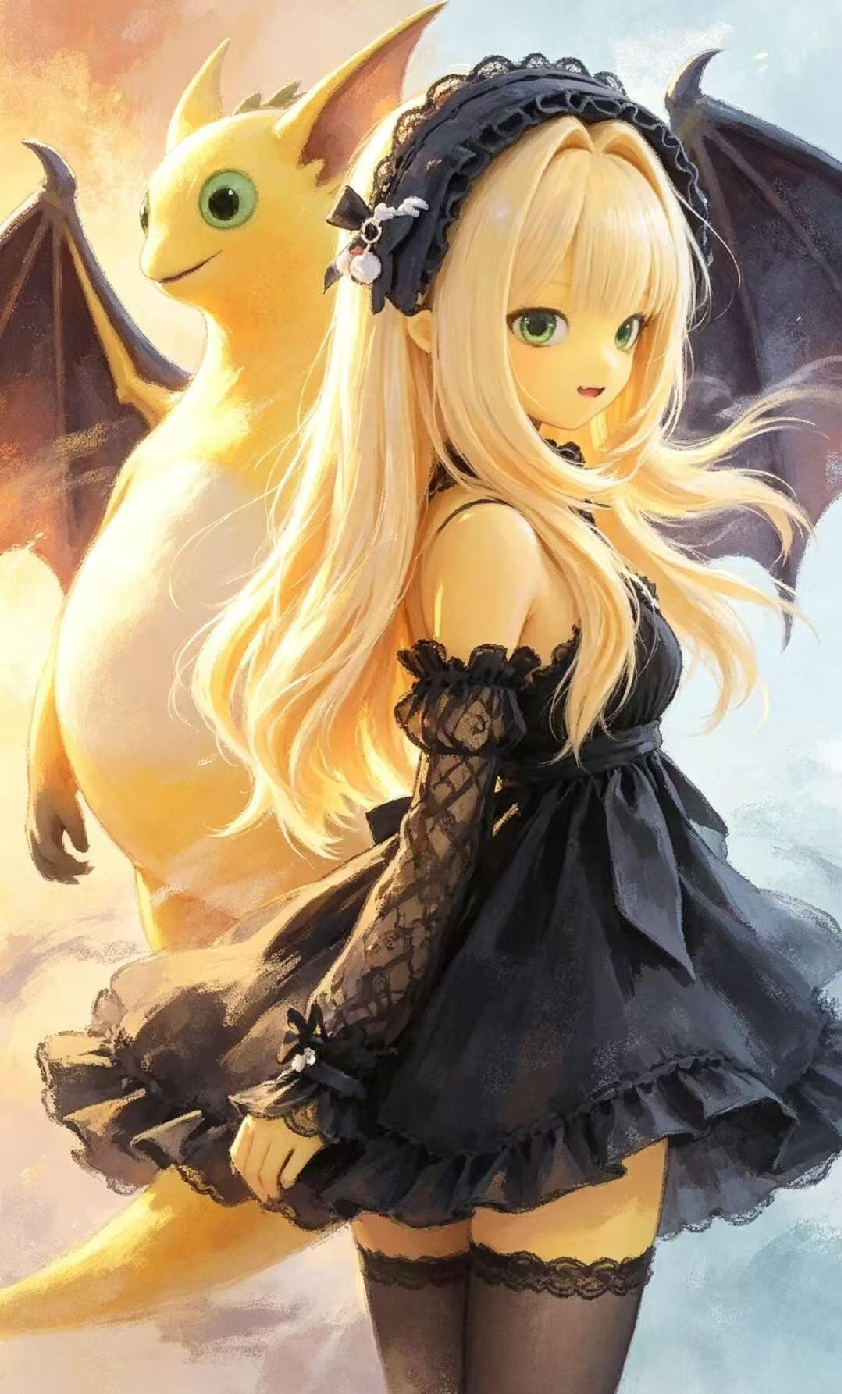
\includegraphics[width=340bp,height=0.90\textheight,keepaspectratio]{figures/chapter07/batPlate.pdf}
  \caption*{奶蝠的真身——美丽诱惑下的奶之恶魔}
\end{figure}
\clearpage



\clearpage
% !TEX root = ../main.tex

\clearpage
% Source PDF page 23.
\section{第八章\quad 奶蛙周边的售卖壮大}

随着奶蛙的爆火，紧随抽象潮流的商家们也纷纷上架奶蛙周边。~(见\figref{fig:08-1})

% !TEX root = ../../main.tex
\begin{figure}[H]
  \centering
  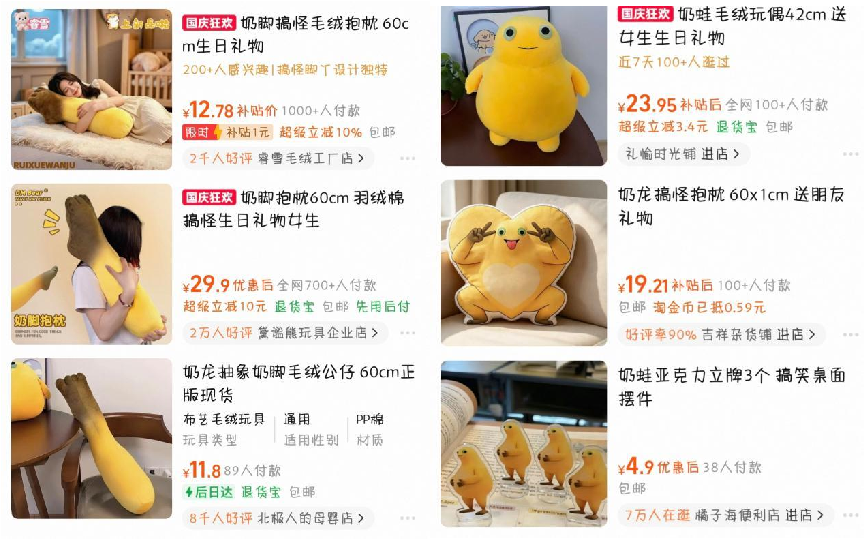
\includegraphics[width=352.85bp,height=0.76\textheight,keepaspectratio]{figures/chapter08/figure08_1.pdf}
  \renewcommand{\thefigure}{8.1}
  \caption{淘宝售卖的奶脚抱枕（左）和奶蛙玩偶、亚克力等（右）}
  \label{fig:08-1}
\end{figure}


% !TEX root = ../../main.tex
\begin{figure}[H]
  \centering
  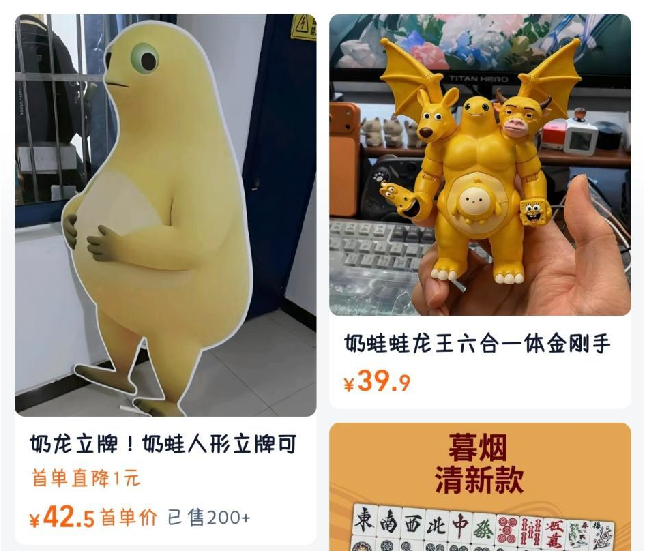
\includegraphics[width=263.3bp,height=0.76\textheight,keepaspectratio]{figures/chapter08/figure08_2.pdf}
  \renewcommand{\thefigure}{8.2}
  \caption{淘宝售卖的 2m 奶蛙人形立牌和奶蛙六合一战神金刚}
  \label{fig:08-2}
\end{figure}


其中最具有影响力的，无疑是奶蛙立牌。各个高校的奶家人不约而同有了一个大胆的想法...我们将会在第九章中具体展开。~(见\figref{fig:08-2})

其中有一些产品无疑是具有新意和实用或观赏价值的。我们将会稍微提及一些有趣的奶味产品。

\clearpage
% Source PDF page 24.
这是淘宝上售卖的奶蛙抽纸盒，由 3D 打印技术制作而成。简单的工艺，不简单的创意。口吐白纸的奶蛙正是笑到极点的表现。~(见\figref{fig:08-3})

% !TEX root = ../../main.tex
\begin{figure}[H]
  \centering
  
\includegraphics[width=83.98bp,height=0.76\textheight,keepaspectratio]{figures/chapter08/figure08_3.pdf}
  \renewcommand{\thefigure}{8.3}
  \caption{奶蛙抽纸盒}
  \label{fig:08-3}
\end{figure}


这是淘宝上售卖的奶味创意奶夜灯，巧妙地运用了阴影的效果，让奶蛙以两种姿态出现在奶民们夜晚的床头。当你夜不能寐的时候，还有奶灯温馨伴你左右。~(见\figref{fig:08-4})

% !TEX root = ../../main.tex
\begin{figure}[H]
  \centering
  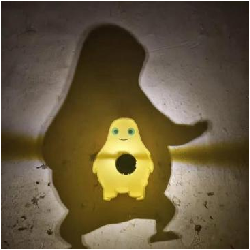
\includegraphics[width=102.03bp,height=0.76\textheight,keepaspectratio]{figures/chapter08/figure08_4.pdf}
  \renewcommand{\thefigure}{8.4}
  \caption{创意奶夜灯，阴影呈现奶蛙的架势}
  \label{fig:08-4}
\end{figure}


这是淘宝上售卖的奶勺子，巧妙地把舌头的形状和勺子联系起来，颇有形体美。\sout{弥补了不能和奶蛙舌吻的遗憾（划去）。}~(见\figref{fig:08-5})

% !TEX root = ../../main.tex
\begin{figure}[H]
  \centering
  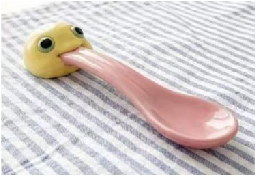
\includegraphics[width=104.38bp,height=0.76\textheight,keepaspectratio]{figures/chapter08/figure08_5.pdf}
  \renewcommand{\thefigure}{8.5}
  \caption{创意奶勺子}
  \label{fig:08-5}
\end{figure}


这是某网购平台上售卖的奶内裤。嗯...有点太神圣了。~(见\figref{fig:08-6})

% !TEX root = ../../main.tex
\begin{figure}[H]
  \centering
  
\includegraphics[width=107.75bp,height=0.76\textheight,keepaspectratio]{figures/chapter08/figure08_6.pdf}
  \renewcommand{\thefigure}{8.6}
  \caption{创意奶内衣}
  \label{fig:08-6}
\end{figure}


\clearpage
% Source PDF page 25.
这是某大学图书馆内的奶蛋椅。学完《奶概》之后惬意地往里面一坐，感觉奶蛙的笑声仿佛回响在耳边一样。~(见\figref{fig:08-7})

% !TEX root = ../../main.tex
\begin{figure}[H]
  \centering
  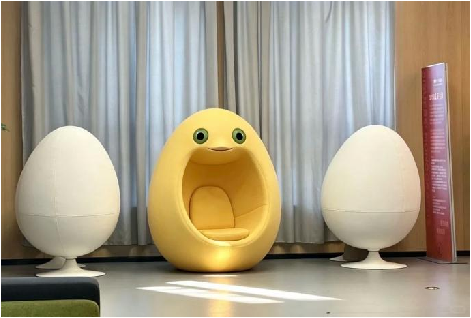
\includegraphics[width=192bp,height=0.76\textheight,keepaspectratio]{figures/chapter08/figure08_7.pdf}
  \renewcommand{\thefigure}{8.7}
  \caption{创意奶蛋椅}
  \label{fig:08-7}
\end{figure}


这是淘宝上售卖的奶蛙假面。戴上它来成为社交悍匪。~(见\figref{fig:08-8})

% !TEX root = ../../main.tex
\begin{figure}[H]
  \centering
  
\includegraphics[width=102.85bp,height=0.76\textheight,keepaspectratio]{figures/chapter08/figure08_8.pdf}
  \renewcommand{\thefigure}{8.8}
  \caption{奶蛙假面}
  \label{fig:08-8}
\end{figure}


这是淘宝上售卖的奶蛙小抱枕。带着小奶蛙周游世界吧。~(见\figref{fig:08-9})

% !TEX root = ../../main.tex
\begin{figure}[H]
  \centering
  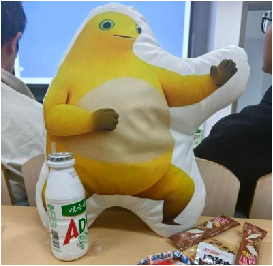
\includegraphics[width=111.52bp,height=0.76\textheight,keepaspectratio]{figures/chapter08/figure08_9.pdf}
  \renewcommand{\thefigure}{8.9}
  \caption{奶蛙小抱枕}
  \label{fig:08-9}
\end{figure}


这是淘宝上售卖的奶蛋小摆件。搭建你自己的奶蛋大军吧！~(见\figref{fig:08-10})

% !TEX root = ../../main.tex
\begin{figure}[H]
  \centering
  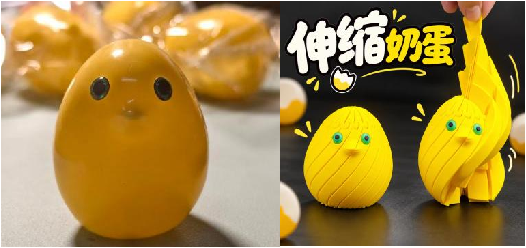
\includegraphics[width=214.74bp,height=0.76\textheight,keepaspectratio]{figures/chapter08/figure08_10.pdf}
  \renewcommand{\thefigure}{8.10}
  \caption{塑料奶蛋小摆件（左）与伸缩奶蛋解压玩具（右）}
  \label{fig:08-10}
\end{figure}



\clearpage
% !TEX root = ../main.tex

\clearpage
% Source PDF page 30.
\section{第九章\quad 奶蛙进校园——高校奶蛙活动概述}

本章将提及一些高校奶蛙活动，不分先后。由于编者精力极度有限，如果读者学校的奶蛙活动未被提及，也请谅解。奶蛙无高低，快乐最重要嘛。

\subsection{一、各自为战的高校奶蛙}

\subsubsection{（1）哈尔滨工业大学}

2026 年 6 月，在哈尔滨工业大学深圳校区的 2026 年毕业典礼暨学位授予仪式上出现了第一个广为人知的奶蛙立牌。哈工大奶蛙立牌的强势出镜破圈，标志着各大学正式进入了奶蛙立牌争先赶超、军备竞赛的阶段的阶段。~(见\figref{fig:09-1})

% !TEX root = ../../main.tex
\begin{figure}[H]
  \centering
  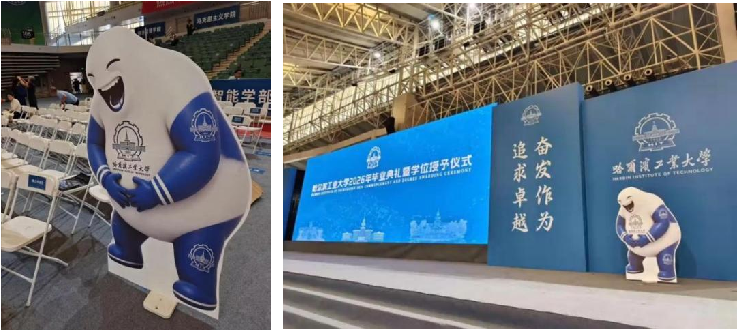
\includegraphics[width=301.14bp,height=0.76\textheight,keepaspectratio]{figures/chapter09/figure09_1.pdf}
  \renewcommand{\thefigure}{9.1}
  \caption{哈尔滨工业大学 2026 年毕业典礼暨学位授予仪式上的奶蛙立牌}
  \label{fig:09-1}
\end{figure}


\subsubsection{（2）武汉大学}

据当前可查询到的信息资料，武汉大学是最早发起流动奶蛙活动的高校（2026/9/12 晚 5 点前后），并且在奶蛙大流动前便拥有千人级别的奶龙群。~(见\figref{fig:09-2})

% !TEX root = ../../main.tex
\begin{figure}[H]
  \centering
  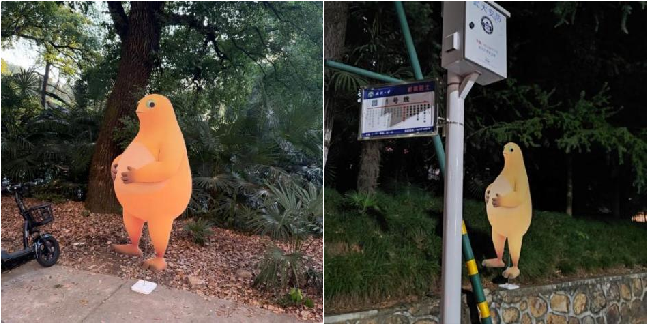
\includegraphics[width=263.19bp,height=0.76\textheight,keepaspectratio]{figures/chapter09/figure09_2.pdf}
  \renewcommand{\thefigure}{9.2}
  \caption{武汉大学的奶蛙立牌的出生点（左）和奶狗气球车（右）}
  \label{fig:09-2}
\end{figure}


在流动奶蛙活动中，同学们可以把奶蛙带到学校各个角落，在任意一处地方偶遇惊喜。这一行为与\textbf{四川农业大学的“搬牛”活动}不谋而合。武大作为流动奶蛙的先驱，为流动奶蛙这一活动打下了范式，揭开了奶蛙立牌时代的序幕。距离较近的华中师范大学与中南财经政法大学紧随其后加入。

\subsubsection{（3）上海交通大学}

上海交通大学集思广益（迫真），紧随武大脚步发起了新一次的大型流动奶蛙活动，并且取得了前所未有的破圈效果。这标志着奶蛙立牌的全面爆火，为奶蛙立牌全面进入校园和奶蛙时代的开启打下了坚实基础。

下为上交最初的流动奶蛙。到本书成书为止仍在使用。~(见\figref{fig:09-3})

\clearpage
% Source PDF page 31.
% !TEX root = ../../main.tex
\begin{figure}[H]
  \centering
  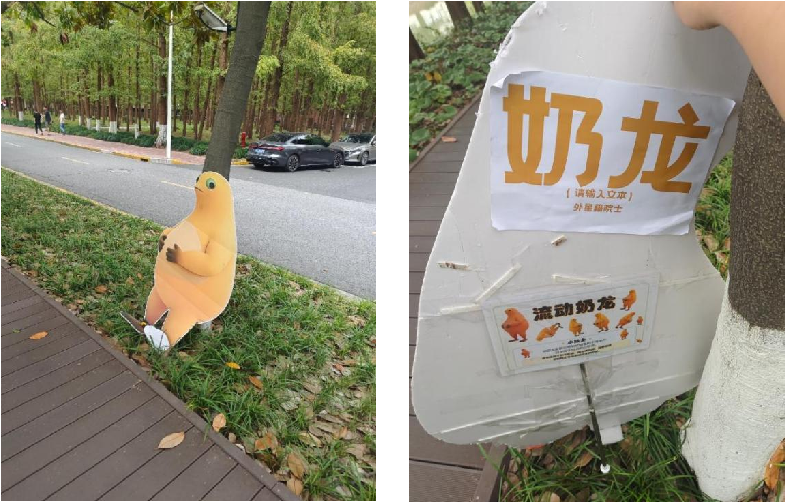
\includegraphics[width=320.62bp,height=0.76\textheight,keepaspectratio]{figures/chapter09/figure09_3.pdf}
  \renewcommand{\thefigure}{9.3}
  \caption{上海交通大学的流动奶蛙立牌}
  \label{fig:09-3}
\end{figure}


\subsubsection{（4）中国海洋大学}

中国海洋大学最为出圈的无疑是“奶 OUC”的四奶蛙立牌。这是第一个广为人知的复数奶蛙立牌，为其他学校提制作更多花样奶蛙立牌打开了思路。~(见\figref{fig:09-4}, \figref{fig:09-5})

% !TEX root = ../../main.tex
\begin{figure}[H]
  \centering
  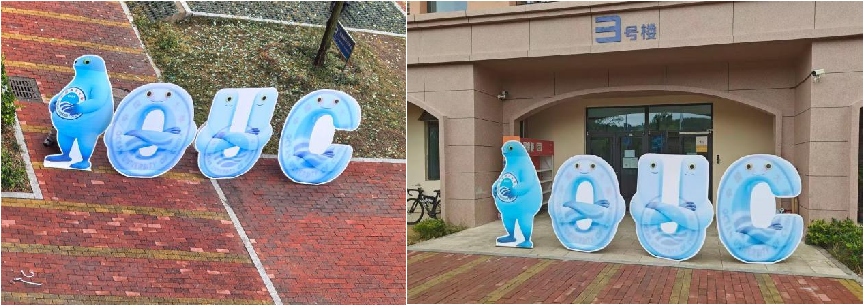
\includegraphics[width=352.34bp,height=0.76\textheight,keepaspectratio]{figures/chapter09/figure09_4.pdf}
  \renewcommand{\thefigure}{9.4}
  \caption{海大的“奶 OUC”四奶蛙立牌}
  \label{fig:09-4}
\end{figure}


% !TEX root = ../../main.tex
\begin{figure}[H]
  \centering
  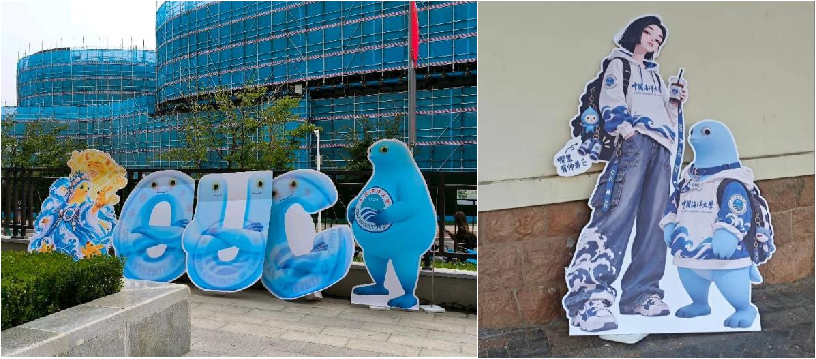
\includegraphics[width=332.96bp,height=0.76\textheight,keepaspectratio]{figures/chapter09/figure09_5.pdf}
  \renewcommand{\thefigure}{9.5}
  \caption{海大奶蛙立牌组完全体形态（左）和绝代双糖（右）}
  \label{fig:09-5}
\end{figure}


\clearpage
% Source PDF page 32.
海大更有院级奶牌，这一思路启发了各高校奶牌的百花齐放。~(见\figref{fig:09-6})

% !TEX root = ../../main.tex
\begin{figure}[H]
  \centering
  
\includegraphics[width=174.05bp,height=0.76\textheight,keepaspectratio]{figures/chapter09/figure09_6.pdf}
  \renewcommand{\thefigure}{9.6}
  \caption{海大行远书院的院级奶龙立牌}
  \label{fig:09-6}
\end{figure}


\subsubsection{（5）浙江大学}

浙江大学在某地的招生宣传立牌中，出现了浙大奶蛙的形象。由于时间无法确定，编者决定将其放在这里。~(见\figref{fig:09-7})

% !TEX root = ../../main.tex
\begin{figure}[H]
  \centering
  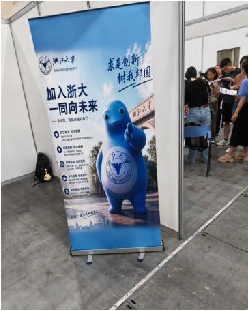
\includegraphics[width=101.63bp,height=0.76\textheight,keepaspectratio]{figures/chapter09/figure09_7.pdf}
  \renewcommand{\thefigure}{9.7}
  \caption{浙大带有奶蛙的招生宣传立牌}
  \label{fig:09-7}
\end{figure}


\subsubsection{（6）北京航空航天大学}

北京航空航天大学的奶龙同好会成立于 2026 年 6 月 24 日。最开始的成立目标是为了让原飞梦社的抽象老登们有个神圣的水群，但是由于奶蛙前所未有的强横热度，人数激增，在 2026 年 8 月初便突破 100 人，在 26 级新生入学后更涌入大量新鲜血液，于 2026 年 9 月 30 日突破 200 人，成为飞梦之后北航校园文化新的中坚力量之一。~(见\figref{fig:09-8})

% !TEX root = ../../main.tex
\begin{figure}[H]
  \centering
  
\includegraphics[width=272.68bp,height=0.76\textheight,keepaspectratio]{figures/chapter09/figure09_8.pdf}
  \renewcommand{\thefigure}{9.8}
  \caption{北航奶龙同好会 100 人贺图（左）及 200 人贺图（右）}
  \label{fig:09-8}
\end{figure}


\clearpage
% Source PDF page 33.
下为 BUAAer 制作的一些北航奶蛙表情包。~(见\figref{fig:09-9})

% !TEX root = ../../main.tex
\begin{figure}[H]
  \centering
  
\includegraphics[width=260.44bp,height=0.76\textheight,keepaspectratio]{figures/chapter09/figure09_9.pdf}
  \renewcommand{\thefigure}{9.9}
  \caption{北航数分奶蛙（左） 捧着航概的奶蛙（中） 校徽奶蛙（右）}
  \label{fig:09-9}
\end{figure}


2026 年 9 月 28 日，一个神秘人在北航学院路校区绿园投放了流动奶蛙立牌。~(见\figref{fig:09-10})

% !TEX root = ../../main.tex
\begin{figure}[H]
  \centering
  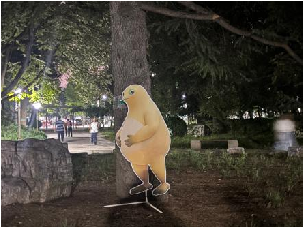
\includegraphics[width=123.86bp,height=0.76\textheight,keepaspectratio]{figures/chapter09/figure09_10.pdf}
  \renewcommand{\thefigure}{9.10}
  \caption{北航学院路校区绿园奶蛙立牌}
  \label{fig:09-10}
\end{figure}


旁边随后还出现了丰川祥子的立牌。学院路的学生们纷纷与之开心合影。~(见\figref{fig:09-11})

% !TEX root = ../../main.tex
\begin{figure}[H]
  \centering
  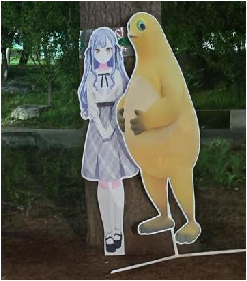
\includegraphics[width=100.81bp,height=0.76\textheight,keepaspectratio]{figures/chapter09/figure09_11.pdf}
  \renewcommand{\thefigure}{9.11}
  \caption{北航学院路校区绿园奶蛙立牌和祥子立牌}
  \label{fig:09-11}
\end{figure}


当晚，奶蛙立牌和祥子立牌被保安发现，立牌被带走，存活约 9 小时。BUAA奶龙同好会对此深表遗憾。下为大家自愿为奶蛙立牌刷屏的一段赞诗：

\begin{center}
\itshape
\fontsize{10.5}{13}\selectfont
我的肉化作黄桃罐头\\
我的血化为蜂蜜\\
我是从天上降下的生活的食粮\\
谁若吃了这食粮\\
必要大笑直到永远\\
我所要赐的食粮\\
就是我的肉\\
为使世界获得笑容。
\end{center}

正因为奶家人的热情，奶蛙在 BUAA 的故事绝不会到此为止。2026 年 10 月2 日，北航沙河校区 TD 线旁出现奶蛙立牌，但被保安迅速逮捕。2026 年 10 月 8日，北航杭州校区出现奶蛙立牌。至此，北航实现了全部校区的奶蛙立牌覆盖。~(见\figref{fig:09-12})

\clearpage
% Source PDF page 34.
% !TEX root = ../../main.tex
\begin{figure}[H]
  \centering
  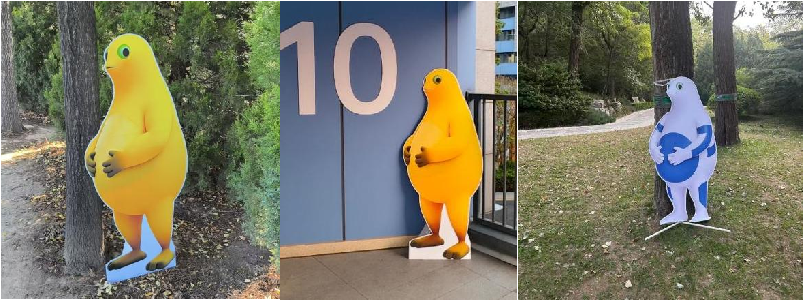
\includegraphics[width=328.17bp,height=0.76\textheight,keepaspectratio]{figures/chapter09/figure09_12.pdf}
  \renewcommand{\thefigure}{9.12}
  \caption{北航沙航奶蛙立牌（左）、杭航奶蛙立牌（中）和学航二代奶蛙立牌（右）}
  \label{fig:09-12}
\end{figure}


2026 年 10 月 9 日，北航沙河校区在 SH2 地下二层的室内完成了全世界首只飞行奶蛙的飞行实现，并取得了完全成功，开创出了北航作为一所航空航天院校的独有奶蛙之路。~(见\figref{fig:09-13})

（飞行奶蛙 B 站视频号：BV1gnps6LEF3）

% !TEX root = ../../main.tex
\begin{figure}[H]
  \centering
  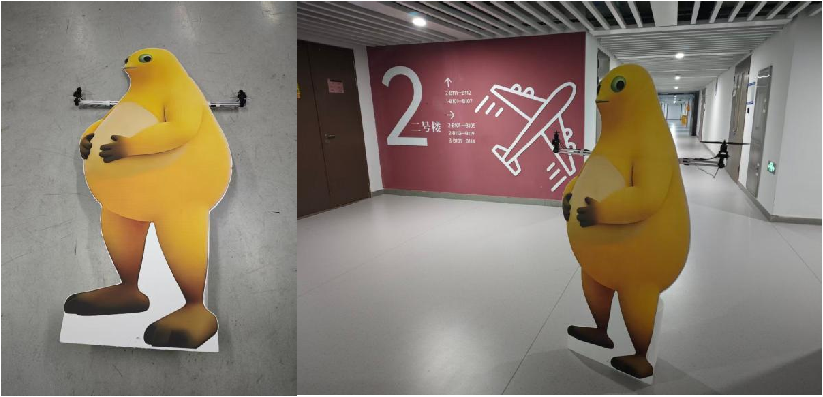
\includegraphics[width=335.92bp,height=0.76\textheight,keepaspectratio]{figures/chapter09/figure09_13.pdf}
  \renewcommand{\thefigure}{9.13}
  \caption{北航沙河校区首只飞行奶蛙试飞现场}
  \label{fig:09-13}
\end{figure}


2026 年 10 月 16 日，BUAA 奶龙同好会出品了奶科学与大笑工程学院培养方案，并绘制了徽标，为可能的奶教学事业画好了蓝图。~(见\figref{fig:09-14})

% !TEX root = ../../main.tex
\begin{figure}[H]
  \centering
  
\includegraphics[width=150.28bp,height=0.76\textheight,keepaspectratio]{figures/chapter09/figure09_14.pdf}
  \renewcommand{\thefigure}{9.14}
  \caption{北航奶龙同好会的奶科学与大笑工程学院标志}
  \label{fig:09-14}
\end{figure}


\clearpage
% Source PDF page 35.
\subsubsection{（7）广东海洋大学}

作为最早一批的奶蛙立牌开拓者，广海的奶蛙立牌在网上同样引发了巨大的反响。谁不想在军训期间被一只奶蛙陪着呢？~(见\figref{fig:09-15})

% !TEX root = ../../main.tex
\begin{figure}[H]
  \centering
  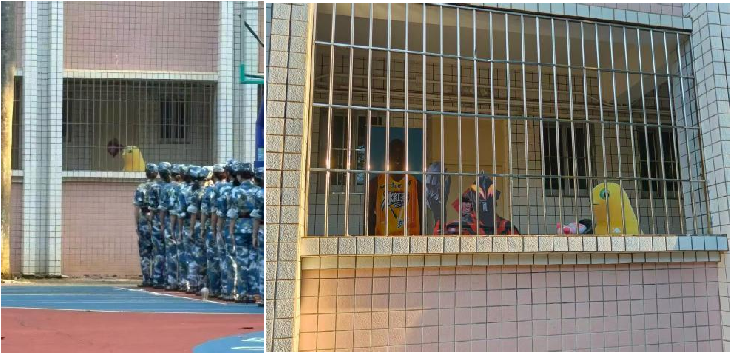
\includegraphics[width=298.38bp,height=0.76\textheight,keepaspectratio]{figures/chapter09/figure09_15.pdf}
  \renewcommand{\thefigure}{9.15}
  \caption{广海的军训奶蛙立牌（左）和“一门四至尊”（右）}
  \label{fig:09-15}
\end{figure}


\subsubsection[（8）南方科技大学]{（8）南方科技大学~(见\figref{fig:09-16})}

% !TEX root = ../../main.tex
\begin{figure}[H]
  \centering
  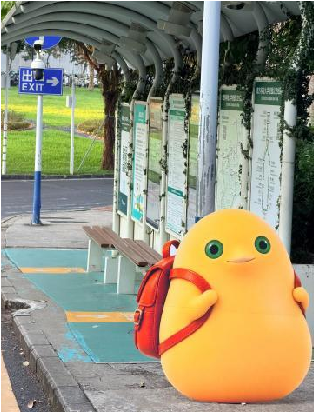
\includegraphics[width=128.45bp,height=0.76\textheight,keepaspectratio]{figures/chapter09/figure09_16.pdf}
  \renewcommand{\thefigure}{9.16}
  \caption{南科大公交站点的奶蛋立牌}
  \label{fig:09-16}
\end{figure}


\subsubsection[（9）山东大学]{（9）山东大学~(见\figref{fig:09-17})}

% !TEX root = ../../main.tex
\begin{figure}[H]
  \centering
  
\includegraphics[width=211.17bp,height=0.76\textheight,keepaspectratio]{figures/chapter09/figure09_17.pdf}
  \renewcommand{\thefigure}{9.17}
  \caption{山大的大笑奶蛙立牌和抱胸奶蛙立牌}
  \label{fig:09-17}
\end{figure}


\clearpage
% Source PDF page 36.
\subsubsection{（10）华中科技大学}~(见\figref{fig:09-18})

% !TEX root = ../../main.tex
\begin{figure}[H]
  \centering
  
\includegraphics[width=117.74bp,height=0.76\textheight,keepaspectratio]{figures/chapter09/figure09_18.pdf}
  \renewcommand{\thefigure}{9.18}
  \caption{华科的左右护法大笑奶蛙立牌}
  \label{fig:09-18}
\end{figure}


2026 年 10 月 10 日，由于华中科技大学奶蛙同好会高层犯下了严重错误，大量华科奶蛙同好会成员对华科奶龙同好会进行爆破，使双方爆发激烈冲突，最终直接导致首届华科奶蛙同好会的解散。对奶龙奶蛙的错误思想使华科的奶龙奶蛙运动受到重创，值得各高校的奶民深思。

\subsubsection[（11）复旦大学]{（11）复旦大学~(见\figref{fig:09-19}, \figref{fig:09-20})}

% !TEX root = ../../main.tex
\begin{figure}[H]
  \centering
  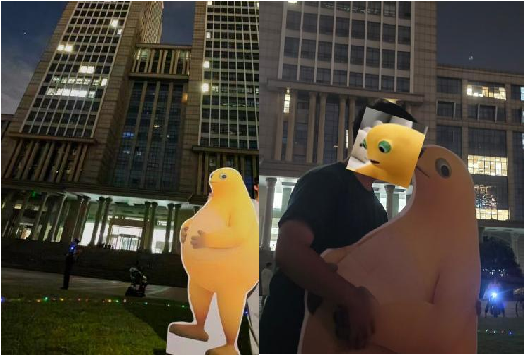
\includegraphics[width=214.13bp,height=0.76\textheight,keepaspectratio]{figures/chapter09/figure09_19.pdf}
  \renewcommand{\thefigure}{9.19}
  \caption{复旦学子与奶蛙立牌激情合照}
  \label{fig:09-19}
\end{figure}


% !TEX root = ../../main.tex
\begin{figure}[H]
  \centering
  
\includegraphics[width=210.56bp,height=0.76\textheight,keepaspectratio]{figures/chapter09/figure09_20.pdf}
  \renewcommand{\thefigure}{9.20}
  \caption{进军复旦百团活动的奶蛙立牌}
  \label{fig:09-20}
\end{figure}


\clearpage
% Source PDF page 37.
\subsubsection{（12）清华大学}

清华变“清蛙”，清华门的沦陷，昭示着奶蛙的大手已经无处不在。~(见\figref{fig:09-21}, \figref{fig:09-22})

% !TEX root = ../../main.tex
\begin{figure}[H]
  \centering
  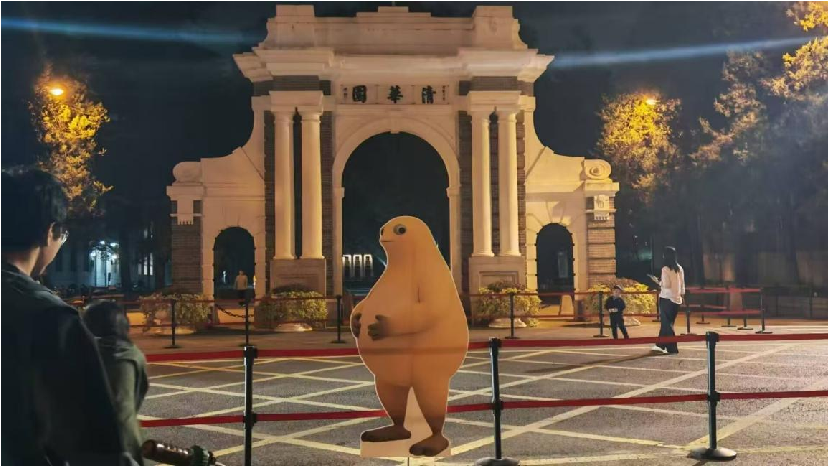
\includegraphics[width=338.27bp,height=0.76\textheight,keepaspectratio]{figures/chapter09/figure09_21.pdf}
  \renewcommand{\thefigure}{9.21}
  \caption{奶蛙占领清华门}
  \label{fig:09-21}
\end{figure}


% !TEX root = ../../main.tex
\begin{figure}[H]
  \centering
  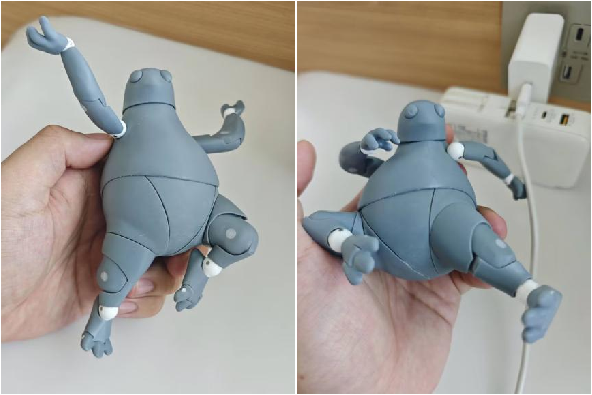
\includegraphics[width=241.47bp,height=0.76\textheight,keepaspectratio]{figures/chapter09/figure09_22.pdf}
  \renewcommand{\thefigure}{9.22}
  \caption{清华学生制作的高自由度可动奶蛙手办}
  \label{fig:09-22}
\end{figure}


\subsubsection[（13）北京理工大学]{（13）北京理工大学~(见\figref{fig:09-23}, \figref{fig:09-24}, \figref{fig:09-25})}

% !TEX root = ../../main.tex
\begin{figure}[H]
  \centering
  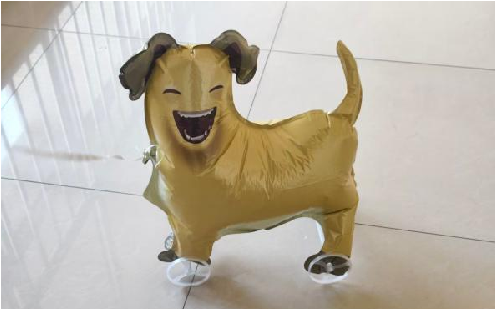
\includegraphics[width=202.5bp,height=0.76\textheight,keepaspectratio]{figures/chapter09/figure09_23.pdf}
  \renewcommand{\thefigure}{9.23}
  \caption{北理的奶狗气球车}
  \label{fig:09-23}
\end{figure}


\clearpage
% Source PDF page 38.
% !TEX root = ../../main.tex
\begin{figure}[H]
  \centering
  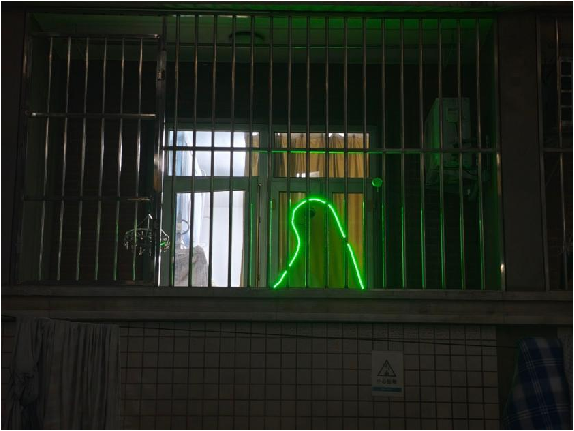
\includegraphics[width=234.12bp,height=0.76\textheight,keepaspectratio]{figures/chapter09/figure09_24.pdf}
  \renewcommand{\thefigure}{9.24}
  \caption{北理的夜光奶蛙}
  \label{fig:09-24}
\end{figure}


% !TEX root = ../../main.tex
\begin{figure}[H]
  \centering
  
\includegraphics[width=128.45bp,height=0.76\textheight,keepaspectratio]{figures/chapter09/figure09_25.pdf}
  \renewcommand{\thefigure}{9.25}
  \caption{北理的奶味校徽“北蛙理工大学”}
  \label{fig:09-25}
\end{figure}


\subsubsection[（14）电子科技大学]{（14）电子科技大学~(见\figref{fig:09-26})}

% !TEX root = ../../main.tex
\begin{figure}[H]
  \centering
  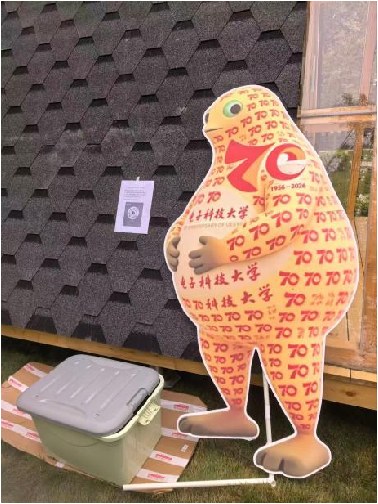
\includegraphics[width=154.36bp,height=0.76\textheight,keepaspectratio]{figures/chapter09/figure09_26.pdf}
  \renewcommand{\thefigure}{9.26}
  \caption{电科的花龙立牌}
  \label{fig:09-26}
\end{figure}


\clearpage
% Source PDF page 39.
\subsubsection{（15）辽宁工程技术大学}

% !TEX root = ../../main.tex
\begin{figure}[H]
  \centering
  
\includegraphics[width=281.15bp,height=0.76\textheight,keepaspectratio]{figures/chapter09/figure09_27.pdf}
  \renewcommand{\thefigure}{9.27}
  \caption{辽工大的原味校徽（左）和奶味校徽（右）}
  \label{fig:09-27}
\end{figure}


辽工大作为校徽上自带两个奶蛙形状的大学，在网上很早便有了名气，一直被人们津津乐道。~(见\figref{fig:09-27})

\subsubsection[（16）中国科学院大学]{（16）中国科学院大学~(见\figref{fig:09-28})}

% !TEX root = ../../main.tex
\begin{figure}[H]
  \centering
  
\includegraphics[width=259.11bp,height=0.76\textheight,keepaspectratio]{figures/chapter09/figure09_28.pdf}
  \renewcommand{\thefigure}{9.28}
  \caption{国科的奶味徽标（左）和国科大的奶龙科学院大学网址（右）}
  \label{fig:09-28}
\end{figure}


\subsubsection[（17）同济大学]{（17）同济大学~(见\figref{fig:09-29})}

% !TEX root = ../../main.tex
\begin{figure}[H]
  \centering
  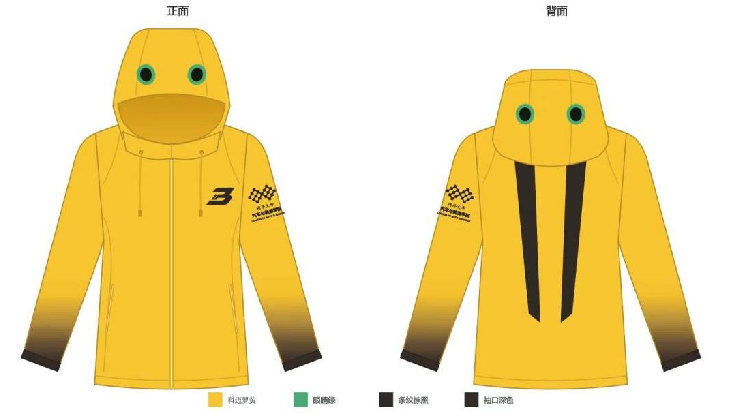
\includegraphics[width=297.98bp,height=0.76\textheight,keepaspectratio]{figures/chapter09/figure09_29.pdf}
  \renewcommand{\thefigure}{9.29}
  \caption{同济材料学院的奶味队服设计概念图}
  \label{fig:09-29}
\end{figure}


\clearpage
% Source PDF page 40.
\subsubsection{（18）北京大学}

% !TEX root = ../../main.tex
\begin{figure}[H]
  \centering
  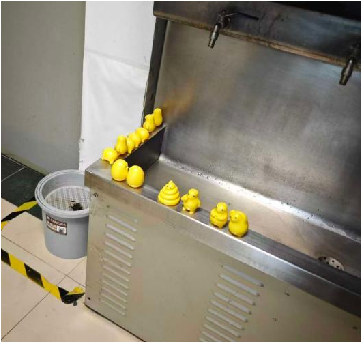
\includegraphics[width=147.83bp,height=0.76\textheight,keepaspectratio]{figures/chapter09/figure09_30.pdf}
  \renewcommand{\thefigure}{9.30}
  \caption{北大放满奶味手办的饮水机}
  \label{fig:09-30}
\end{figure}


值得惋惜的是，同为 Top2 的 PKU 没有像 THU 一样开放，而是对奶蛙进行了严密封锁。即使在宿舍内部张贴奶蛙相关贴画、摆放立牌也会被检查没收，在校内论坛发奶蛙/奶龙字样大概率就会被封禁。~(见\figref{fig:09-30})

\subsubsection[（19）北京师范大学]{（19）北京师范大学~(见\figref{fig:09-31})}

% !TEX root = ../../main.tex
\begin{figure}[H]
  \centering
  
\includegraphics[width=250.04bp,height=0.76\textheight,keepaspectratio]{figures/chapter09/figure09_31.pdf}
  \renewcommand{\thefigure}{9.31}
  \caption{从北师大浴室洗完澡的奶蛙}
  \label{fig:09-31}
\end{figure}


\subsubsection[（20）北京农学院]{（20）北京农学院~(见\figref{fig:09-32})}

% !TEX root = ../../main.tex
\begin{figure}[H]
  \centering
  
\includegraphics[width=112.34bp,height=0.76\textheight,keepaspectratio]{figures/chapter09/figure09_32.pdf}
  \renewcommand{\thefigure}{9.32}
  \caption{北农憨态可掬的奶蛙形象}
  \label{fig:09-32}
\end{figure}


\clearpage
% Source PDF page 41.
\subsubsection{（21）兰州大学}~(见\figref{fig:09-33})

% !TEX root = ../../main.tex
\begin{figure}[H]
  \centering
  
\includegraphics[width=144.98bp,height=0.76\textheight,keepaspectratio]{figures/chapter09/figure09_33.pdf}
  \renewcommand{\thefigure}{9.33}
  \caption{兰大的奶蛙立牌}
  \label{fig:09-33}
\end{figure}


\subsubsection[（22）东北师范大学]{（22）东北师范大学~(见\figref{fig:09-34})}

% !TEX root = ../../main.tex
\begin{figure}[H]
  \centering
  
\includegraphics[width=282.37bp,height=0.76\textheight,keepaspectratio]{figures/chapter09/figure09_34.pdf}
  \renewcommand{\thefigure}{9.34}
  \caption{东北师大的奶龙文化传播研究所牌}
  \label{fig:09-34}
\end{figure}


\subsubsection[（23）上海理工大学]{（23）上海理工大学~(见\figref{fig:09-35})}

% !TEX root = ../../main.tex
\begin{figure}[H]
  \centering
  
\includegraphics[width=228.62bp,height=0.76\textheight,keepaspectratio]{figures/chapter09/figure09_35.pdf}
  \renewcommand{\thefigure}{9.35}
  \caption{上海理工大学的 120 周年校庆奶蛙立牌}
  \label{fig:09-35}
\end{figure}


\clearpage
% Source PDF page 42.
\subsection{二、前所未有的高校线上奶蛙大热潮}

2026 年 10 月 9 日，为促进各高校之间抑制不住的奶蛙热情，各高校之前成立了众多跨高校奶蛙群，如“世界奶蛙联合组织”群（简称世蛙会）、“各高校奶龙联合会”、“高校奶龙同好会”等，并且在各个高校的奶龙同好群之间互相传播各自奶龙同好会的群号，使得各个高校的奶龙同好会达到了空前绝后的规模。~(见\figref{fig:09-36})

% !TEX root = ../../main.tex
\begin{figure}[H]
  \centering
  
\includegraphics[width=133.04bp,height=0.76\textheight,keepaspectratio]{figures/chapter09/figure09_36.pdf}
  \renewcommand{\thefigure}{9.36}
  \caption{“世蛙会”的吉祥物奶蛙}
  \label{fig:09-36}
\end{figure}


在这股前所未有的热潮下，奶蛙旗帜被确定下来。奶蛙旗帜为整体黄色、中心有一绿一黑同心圆的旗帜，形成奶蛙一只眼睛的图案。奶蛙旗帜没有必须的尺寸比例限制。~(见\figref{fig:09-37})

% !TEX root = ../../main.tex
\begin{figure}[H]
  \centering
  
\includegraphics[width=118.15bp,height=0.76\textheight,keepaspectratio]{figures/chapter09/figure09_37.pdf}
  \renewcommand{\thefigure}{9.37}
  \caption{方形奶蛙旗帜}
  \label{fig:09-37}
\end{figure}


由此，奶国这一假想国家的概念基本形成。热爱奶龙、奶蛙的人可以开玩笑般地自称为奶国居民。

\clearpage
% Source PDF page 43.
% !TEX root = ../../main.tex
\clearpage
\begin{figure}[H]
  \centering
  \phantomsection
  \addcontentsline{lof}{figure}{\protect\numberline{}世蛙会成立，奶蛙在奶蛙旗帜下向现实中的大家行礼}
  
\includegraphics[width=353.57bp,height=0.90\textheight,keepaspectratio]{figures/chapter09/flagPlate.pdf}
  \caption*{世蛙会成立，奶蛙在奶蛙旗帜下向现实中的大家行礼}
\end{figure}

\clearpage


\clearpage
% Source PDF page 44.
% !TEX root = ../../main.tex
\clearpage
\begin{figure}[H]
  \centering
  \phantomsection
  \addcontentsline{lof}{figure}{\protect\numberline{}2026 年 10 月 12 日，北航奶龙同好会正式突破 1000 龙}
  
\includegraphics[width=324.7bp,height=0.90\textheight,keepaspectratio]{figures/chapter09/buaaPlate.pdf}
  \caption*{2026 年 10 月 12 日，北航奶龙同好会正式突破 1000 龙}
\end{figure}

\clearpage



\clearpage
% !TEX root = ../main.tex

\clearpage
% Source PDF page 45.
\section{第十章\quad 国际奶蛙传播人士}

在本章，我们将会了解一些致力于在国际平台传播奶蛙文化的人士和大学，或者本身被冠以奶之名的人士。

\textbf{【免责声明】}本章信息来源均来自于国内网络平台及聊天平台的流传图，渠道合法合规。请不要为了一睹国际奶蛙传播人士的风采而擅自使用违规工具进行违法网络活动。\textbf{若读者明知故犯，因此被抓获受到法律处罚，本书不承担包括但不限于诱导、教唆犯罪等相关法律责任。}~(见\figref{fig:10-1})

% !TEX root = ../../main.tex
\begin{figure}[H]
  \centering
  
\includegraphics[width=104.48bp,height=0.76\textheight,keepaspectratio]{figures/chapter10/figure10_1.pdf}
  \renewcommand{\thefigure}{10.1}
  \caption{奶察在看着你...}
  \label{fig:10-1}
\end{figure}


\subsubsection{（1）灰}

% !TEX root = ../../main.tex
\begin{figure}[H]
  \centering
  
\includegraphics[width=351.83bp,height=0.76\textheight,keepaspectratio]{figures/chapter10/figure10_2.pdf}
  \renewcommand{\thefigure}{10.2}
  \caption{灰的 X（原推特）账号主页和被转到国内平台的相关推文}
  \label{fig:10-2}
\end{figure}


灰，奶国公民编号 000001，是一名奶蛙抽象大师。~(见\figref{fig:10-2})

他在 X 上高频率发送高质量 AI 奶蛙图文，并且自发为奶民提供奶国公民证编号（虽然概率很小啊，也可能是抽象的帽子叔叔利用 X 的关注可追溯性钓鱼）。其制作的部分图片或唯美（如一顿简单典雅的奶早餐、奶龙独自在美景中荡秋千）、

\clearpage
% Source PDF page 46.
\noindent 或科学（如《远古奶蛙灭绝事件研究：最后 24 小时》、《远古巨型奶蛙化石的发现及其演化意义》、《史前洞穴岩画中的奶蛙形象及其与早期人类的共存证据研究》等）。这些极具创造力的图片无疑为奶蛙的国内循环传播及对国外输出起到了极为重要的作用。~(见\figref{fig:10-3}, \figref{fig:10-4})

% !TEX root = ../../main.tex
\begin{figure}[H]
  \centering
  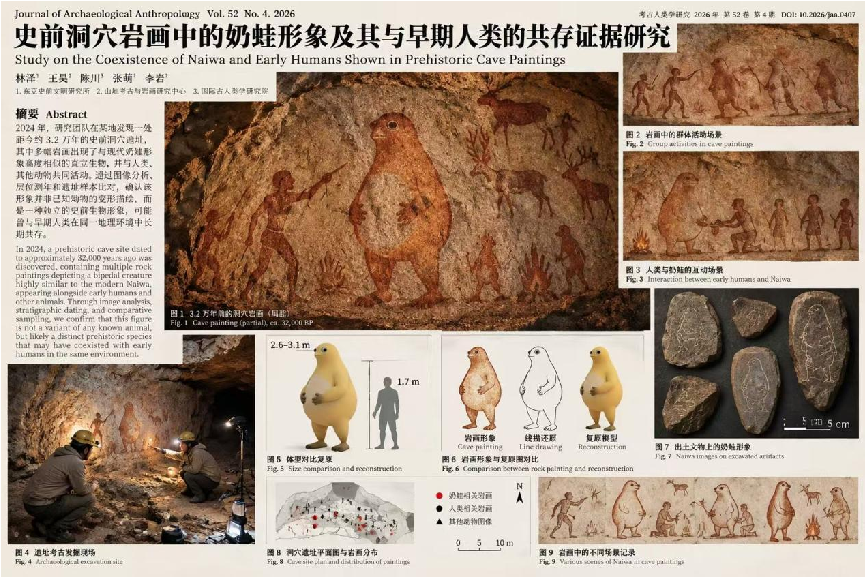
\includegraphics[width=353.36bp,height=0.76\textheight,keepaspectratio]{figures/chapter10/figure10_3.pdf}
  \renewcommand{\thefigure}{10.3}
  \caption{灰制作的一张奶蛙伪科学图解}
  \label{fig:10-3}
\end{figure}


% !TEX root = ../../main.tex
\begin{figure}[H]
  \centering
  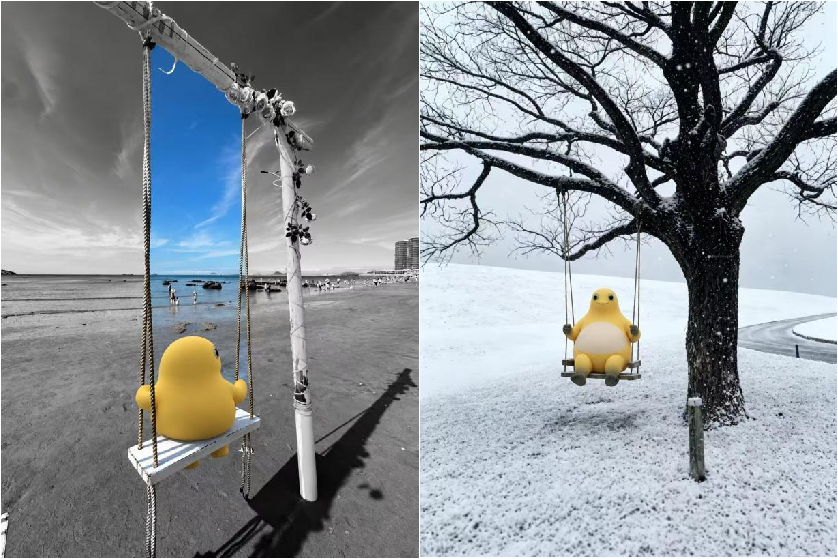
\includegraphics[width=342.04bp,height=0.76\textheight,keepaspectratio]{figures/chapter10/figure10_4.pdf}
  \renewcommand{\thefigure}{10.4}
  \caption{灰制作的两张极有意境的奶蛙秋千图}
  \label{fig:10-4}
\end{figure}


\subsubsection{（2）唐纳德·特朗普}

川宝，美国第 45、第 47 任美国总统，因为其金色的头发、极具张力的手风琴手势和捉摸不透的行政风格，被国内称别名为“奶龙”（被冠以奶之名の男）。~(见\figref{fig:10-5})

\clearpage
% Source PDF page 47.
% !TEX root = ../../main.tex
\begin{figure}[H]
  \centering
  
\includegraphics[width=131.41bp,height=0.76\textheight,keepaspectratio]{figures/chapter10/figure10_5.pdf}
  \renewcommand{\thefigure}{10.5}
  \caption{特朗普形象的奶蛙}
  \label{fig:10-5}
\end{figure}


\subsubsection{（3）埃隆·马斯克}

可能是因为 X 对用户账号的误封过于离谱，名字里又正好带个“隆”字，马斯克和奶家不知怎么地就莫名其妙地扯上了关系，变成了“奶隆”。~(见\figref{fig:10-6})

% !TEX root = ../../main.tex
\begin{figure}[H]
  \centering
  
\includegraphics[width=111bp,height=0.76\textheight,keepaspectratio]{figures/chapter10/figure10_6.pdf}
  \renewcommand{\thefigure}{10.6}
  \caption{奶隆正在对 X 用户封号中}
  \label{fig:10-6}
\end{figure}


\subsubsection{（4）将军}

黑衣背头，捧腹大笑，这就是奶化二创里的“将军”。~(见\figref{fig:10-7})

% !TEX root = ../../main.tex
\begin{figure}[H]
  \centering
  
\includegraphics[width=68bp]{figures/chapter10/figure10_7.png}
  \renewcommand{\thefigure}{10.7}
  \caption{捧腹大笑的将军（二创）}
  \label{fig:10-7}
\end{figure}


\subsubsection[（5）密歇根大学]{（5）密歇根大学~(见\figref{fig:10-8})}

% !TEX root = ../../main.tex
\begin{figure}[H]
  \centering
  
\includegraphics[width=154.87bp,height=0.76\textheight,keepaspectratio]{figures/chapter10/figure10_8.pdf}
  \renewcommand{\thefigure}{10.8}
  \caption{威斯康星大学麦迪逊分校的奶蛙形象}
  \label{fig:10-8}
\end{figure}


\clearpage
% Source PDF page 48.
\subsubsection[（6）威斯康星大学]{（6）威斯康星大学~(见\figref{fig:10-9})}

% !TEX root = ../../main.tex
\begin{figure}[H]
  \centering
  
\includegraphics[width=310.01bp,height=0.76\textheight,keepaspectratio]{figures/chapter10/figure10_9.pdf}
  \renewcommand{\thefigure}{10.9}
  \caption{纽约大学校徽（左）和身穿紫衣的 NYU 奶蛙立牌（右）}
  \label{fig:10-9}
\end{figure}


\subsubsection[（7）纽约大学]{（7）纽约大学~(见\figref{fig:10-10})}

% !TEX root = ../../main.tex
\begin{figure}[H]
  \centering
  
\includegraphics[width=188.43bp,height=0.76\textheight,keepaspectratio]{figures/chapter10/figure10_10.pdf}
  \renewcommand{\thefigure}{10.10}
  \caption{贴在柱子上的 UoA 奶蛙宣传单}
  \label{fig:10-10}
\end{figure}


\subsubsection[（8）奥克兰大学]{（8）奥克兰大学~(见\figref{fig:10-11})}

% !TEX root = ../../main.tex
\begin{figure}[H]
  \centering
  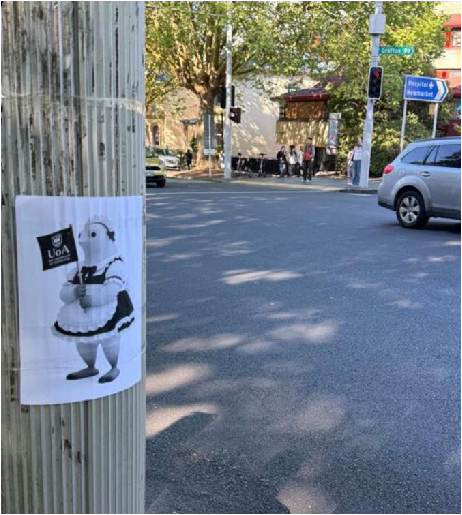
\includegraphics[width=188.43bp,height=0.76\textheight,keepaspectratio]{figures/chapter10/figure10_11.pdf}
  \renewcommand{\thefigure}{10.11}
  \caption{贴在柱子上的 UoA 奶蛙宣传单}
  \label{fig:10-11}
\end{figure}


\clearpage
% !TEX root = ../main.tex

\clearpage
% Source PDF page 49.
\section{第十一章\quad 奶科学简介}

在奶蛙的热潮下，各个领域纷纷乱入奶蛙，形成了看似一本正经实则奇异搞笑的奶科学。本章将对几个领域形成的奶科学进行简单介绍。

\subsection{一、奶数学}

奶数学，顾名思义，就是用各种数学的方式表现出奶蛙。在数学分析和工程领域，傅里叶变换能够将一个复杂的图形用三角函数无限逼近模拟。因此，许多大学生使用傅里叶级数来绘制奶蛙。~(见\figref{fig:11-1})

% !TEX root = ../../main.tex
\begin{figure}[H]
  \centering
  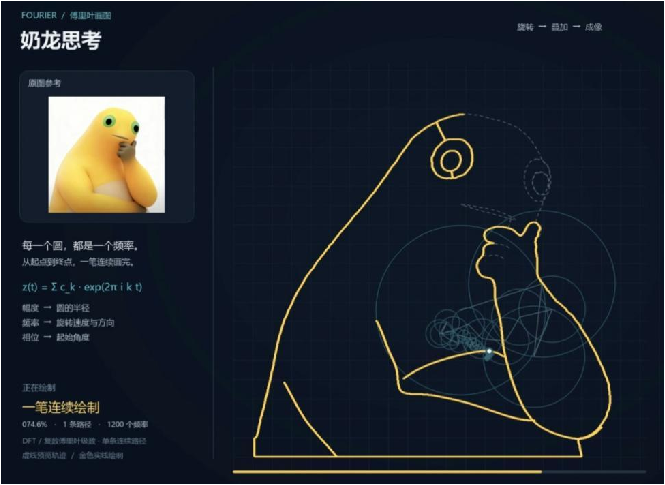
\includegraphics[width=271.15bp,height=0.76\textheight,keepaspectratio]{figures/chapter11/figure11_1.pdf}
  \renewcommand{\thefigure}{11.1}
  \caption{使用傅里叶级数一笔绘制思考奶蛙}
  \label{fig:11-1}
\end{figure}


同理，其他的曲线也可以构成奶蛙。~(见\figref{fig:11-2}, \figref{fig:11-3})

% !TEX root = ../../main.tex
\begin{figure}[H]
  \centering
  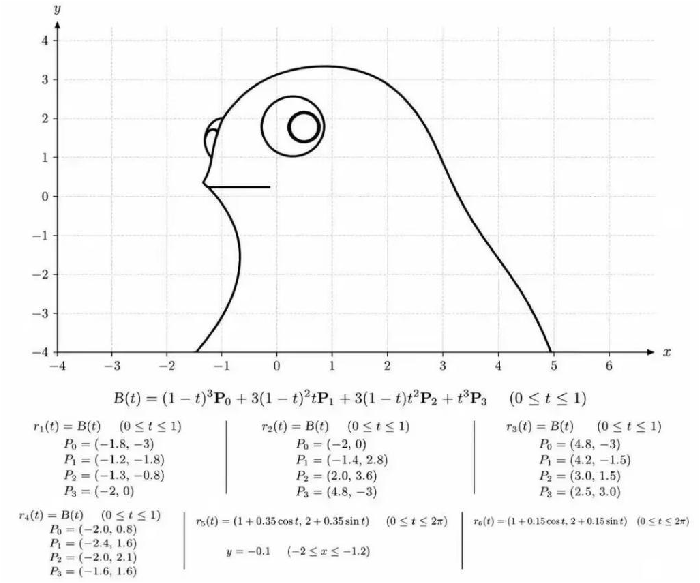
\includegraphics[width=285.43bp,height=0.76\textheight,keepaspectratio]{figures/chapter11/figure11_2.pdf}
  \renewcommand{\thefigure}{11.2}
  \caption{奶蛙曲线}
  \label{fig:11-2}
\end{figure}


\clearpage
% Source PDF page 50.
% !TEX root = ../../main.tex
\begin{figure}[H]
  \centering
  
\includegraphics[width=340.41bp,height=0.76\textheight,keepaspectratio]{figures/chapter11/figure11_3.pdf}
  \renewcommand{\thefigure}{11.3}
  \caption{恶搞考研题：奶蛙头面积问题}
  \label{fig:11-3}
\end{figure}


\subsection{二、奶语言学}

由于日语中ないわ的罗马音为 na i wa（谐音奶蛙），因此一些耳朵尖的青年使用曾经在网上火过的“仙人指路”法，把一些歌曲中的ないわ圈出来并指向奶蛙，形成了非常搞笑的效果。~(见\figref{fig:11-4})

% !TEX root = ../../main.tex
\begin{figure}[H]
  \centering
  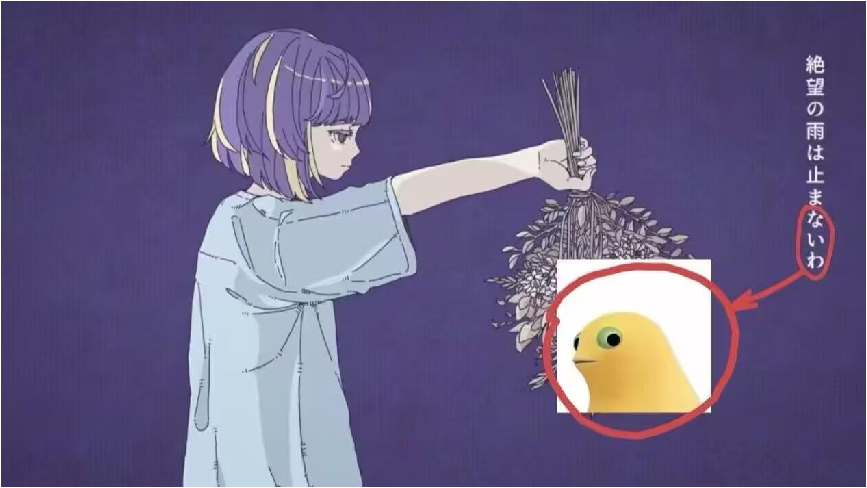
\includegraphics[width=353.77bp,height=0.76\textheight,keepaspectratio]{figures/chapter11/figure11_4.pdf}
  \renewcommand{\thefigure}{11.4}
  \caption{歌曲 phony 中的ないわ}
  \label{fig:11-4}
\end{figure}


\subsection{三、奶艺术学和奶历史学}

将梗糅合进入艺术和历史等通俗文科领域，以取得与现实大致相似却稍有不同的微妙效果，是互联网常见的一种做法。

而对比奶龙更接近于人形、拥有无穷无尽变种的奶蛙在这一点上明显有着巨大的优势。因此，奶蛙形成的奶艺术学和奶历史学拥有无比巨大的规模，给我们带来了一场视觉盛宴。~(见\figref{fig:11-5}, \figref{fig:11-7}, \figref{fig:11-8})

\clearpage
% Source PDF page 51.
% !TEX root = ../../main.tex
\begin{figure}[H]
  \centering
  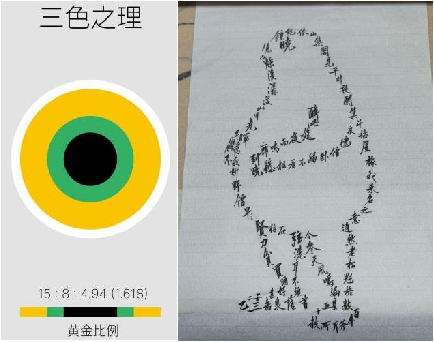
\includegraphics[width=176.9bp,height=0.76\textheight,keepaspectratio]{figures/chapter11/figure11_5.pdf}
  \renewcommand{\thefigure}{11.5}
  \caption{奶蛙黄金比（左）和由潇洒字体围成的奶蛙（右）}
  \label{fig:11-5}
\end{figure}


% !TEX root = ../../main.tex
\begin{figure}[H]
  \centering
  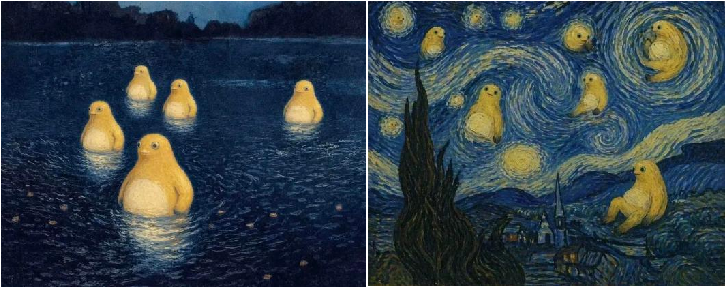
\includegraphics[width=296.24bp,height=0.76\textheight,keepaspectratio]{figures/chapter11/figure11_6.pdf}
  \renewcommand{\thefigure}{11.6}
  \caption{世界名画：河上的奶蛙（左）和奶空（右）}
  \label{fig:11-6}
\end{figure}


《河上的奶蛙》是对挪威著名画家弗里茨·索洛（Frits Thaulow）1880 年作品的模仿奶作，作品描绘了宁静河面上几只优雅的奶蛙，水面映照出周围景物的倒影，营造出神秘而安静的氛围。画面延续了索洛对水景的细腻刻画：深蓝色的水面通过丰富而流动的笔触表现出微妙的波纹变化，反射出环境的朦胧光影。奶蛙以柔和的暖黄色呈现，其圆润的体态在水中形成轻微的倒影与光晕，与周围环境自然融合。艺术家通过对光线的控制，使奶蛙周围的水面略显明亮，既强化了主体，又保持了整体画面的统一与和谐。作为 19 世纪挪威重要的风景画家之一，弗里茨·索洛以擅长描绘自然光线下的水面效果而著称。他的作品常通过细腻的观察与丰富的色彩变化，表现水流的动态与环境的静谧。在《河上的奶蛙》中，这种对水面质感与光影变化的表现依然得以保留，并通过新的形象转化，呈现出一种介于传统自然描绘与当代视觉符号之间的独特效果。~(见\figref{fig:11-6})

% !TEX root = ../../main.tex
\begin{figure}[H]
  \centering
  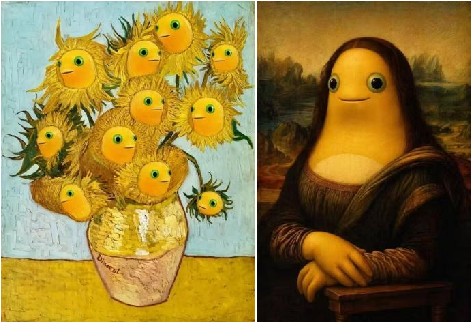
\includegraphics[width=192.41bp,height=0.76\textheight,keepaspectratio]{figures/chapter11/figure11_7.pdf}
  \renewcommand{\thefigure}{11.7}
  \caption{世界名画：向日奶（左）和蒙奶丽莎（右）}
  \label{fig:11-7}
\end{figure}


\clearpage
% Source PDF page 52.
% !TEX root = ../../main.tex
\begin{figure}[H]
  \centering
  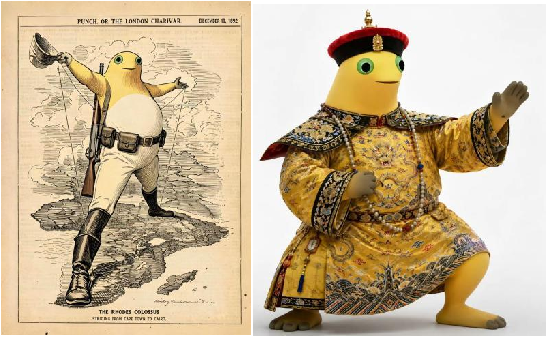
\includegraphics[width=223.31bp,height=0.76\textheight,keepaspectratio]{figures/chapter11/figure11_8.pdf}
  \renewcommand{\thefigure}{11.8}
  \caption{奶蛙在非洲的野心（左）和奶蛙帝国的安迪皇帝（右）}
  \label{fig:11-8}
\end{figure}


\subsection{四、奶烹饪技术学}

众所周知，奶龙的黄颜色和圆滚滚的形体，让人很自然地联想到黄桃罐头。因此，产生了奶龙尸块是黄桃罐头的说法。这一说法继承给了同样黄色、同样肚皮圆滚滚的奶蛙。~(见\figref{fig:11-9})

% !TEX root = ../../main.tex
\begin{figure}[H]
  \centering
  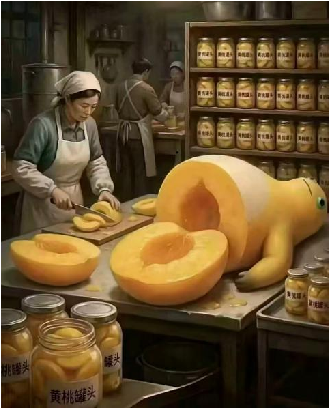
\includegraphics[width=134.78bp,height=0.76\textheight,keepaspectratio]{figures/chapter11/figure11_9.pdf}
  \renewcommand{\thefigure}{11.9}
  \caption{奶蛙被做成“黄桃罐头”}
  \label{fig:11-9}
\end{figure}


这一说法巧妙地给奶蛙加入了可食用的属性。由此，人们开始创作有关食物的奶蛙形象，甚至亲自动手做出吃的到的奶味食品。自此，奶烹饪技术学成为了一门颇为有趣的奶科学。~(见\figref{fig:11-10}, \figref{fig:11-11})

% !TEX root = ../../main.tex
\begin{figure}[H]
  \centering
  
\includegraphics[width=134.78bp,height=0.76\textheight,keepaspectratio]{figures/chapter11/figure11_10.pdf}
  \renewcommand{\thefigure}{11.10}
  \caption{奶蛙被做成“黄桃罐头”}
  \label{fig:11-10}
\end{figure}


\clearpage
% Source PDF page 53.
% !TEX root = ../../main.tex
\begin{figure}[H]
  \centering
  
\includegraphics[width=225.15bp,height=0.76\textheight,keepaspectratio]{figures/chapter11/figure11_11.pdf}
  \renewcommand{\thefigure}{11.11}
  \caption{小红书某博主的手工奶蛋饼干（左）和一些食品商家推出的脆奶皮（右）}
  \label{fig:11-11}
\end{figure}


\subsection{五、奶哲学}

奶蛙一直在捧腹大笑，周而复始。因此，我们必须想象西西弗奶是幸福的。这就是奶哲学告诉我们的道理。奶哲学这一系中有名著《奶托邦》，能够启发我们对不同社会模式和生存方式的反思。我们这里引用几句：~(见\figref{fig:11-12})

奶托邦意为“根本没有的地方”。根本没有这样的地方！——《奶托邦》

我们一度怀疑自己来到了传说中的蜜与奶之地...“安迪！”他们看到我们，就突然抬起头，发出一种嘹亮的叫声。——《奶托邦》

% !TEX root = ../../main.tex
\begin{figure}[H]
  \centering
  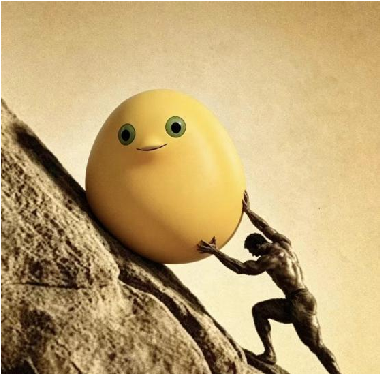
\includegraphics[width=155.38bp,height=0.76\textheight,keepaspectratio]{figures/chapter11/figure11_12.pdf}
  \renewcommand{\thefigure}{11.12}
  \caption{正在搬运奶蛋的西西弗奶}
  \label{fig:11-12}
\end{figure}


\subsection{六、奶政治学与奶法律学}

\textbf{【免责声明】}本节条文为架空内容，\textbf{不具有任何政治、法律效力，没有对现实中任何国家的政治制度和法律进行模仿、影射、亵渎。}不当改动本节内容可能引发不必要的风波，故本书编写组\textbf{不建议其他编写组对此节进行任何改动。若改编者私自在本节内塞入有关现实政治、法律私货进行反动宣传，并因此被抓获受到严厉法律处罚，本书不承担包括但不限于诱导、教唆犯罪等相关法律责任。}

在华科的龙蛙之争结束后，奶家人们意识到了需要一些特定称谓来形容一些影响奶蛙活动的不当行为。于是，一些奶家人开始使用被各种奶化了的罪名和一些俏皮调侃的“处罚”来模拟奶国法律处罚宣判时的可能情景，由此形成了奶法律学的雏形。

例如，如下的“剥夺大笑权利终身”就是奶国的最高惩罚之一。~(见\figref{fig:11-13})

\clearpage
% Source PDF page 54.
% !TEX root = ../../main.tex
\begin{figure}[H]
  \centering
  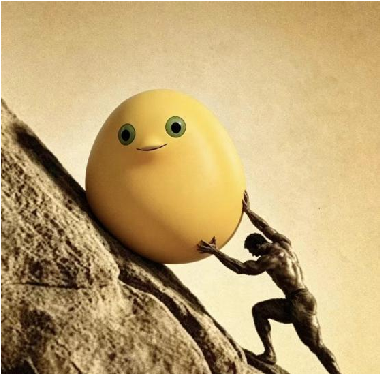
\includegraphics[width=155.38bp,height=0.76\textheight,keepaspectratio]{figures/chapter11/figure11_13.pdf}
  \renewcommand{\thefigure}{11.13}
  \caption{正在搬运奶蛋的西西弗奶}
  \label{fig:11-13}
\end{figure}


\subsection[七、奶工程学]{七、奶工程学~(见\figref{fig:11-14}, \figref{fig:11-15})}

% !TEX root = ../../main.tex
\begin{figure}[H]
  \centering
  
\includegraphics[width=281.55bp,height=0.76\textheight,keepaspectratio]{figures/chapter11/figure11_14.pdf}
  \renewcommand{\thefigure}{11.14}
  \caption{奶蛙模拟电路绘图}
  \label{fig:11-14}
\end{figure}


% !TEX root = ../../main.tex
\begin{figure}[H]
  \centering
  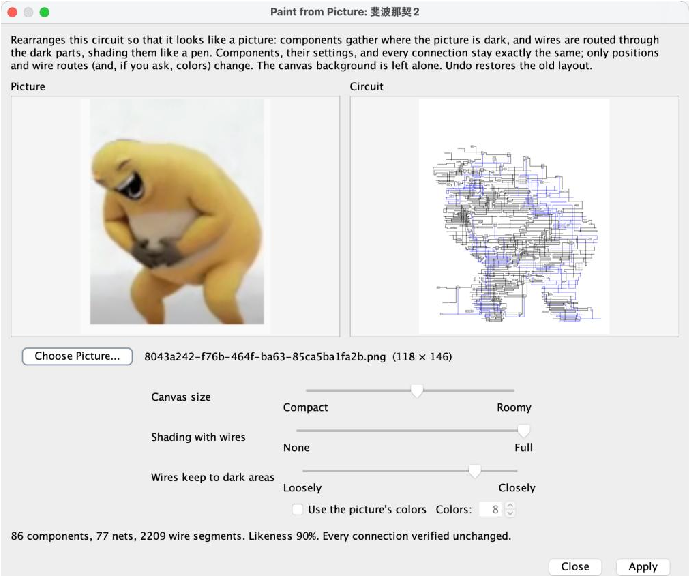
\includegraphics[width=281.55bp,height=0.76\textheight,keepaspectratio]{figures/chapter11/figure11_15.pdf}
  \renewcommand{\thefigure}{11.15}
  \caption{奶蛙模拟电路绘图}
  \label{fig:11-15}
\end{figure}


\clearpage
% Source PDF page 55.
\subsection[八、奶生物学和奶医学]{八、奶生物学和奶医学~(见\figref{fig:11-16})}

% !TEX root = ../../main.tex
\begin{figure}[H]
  \centering
  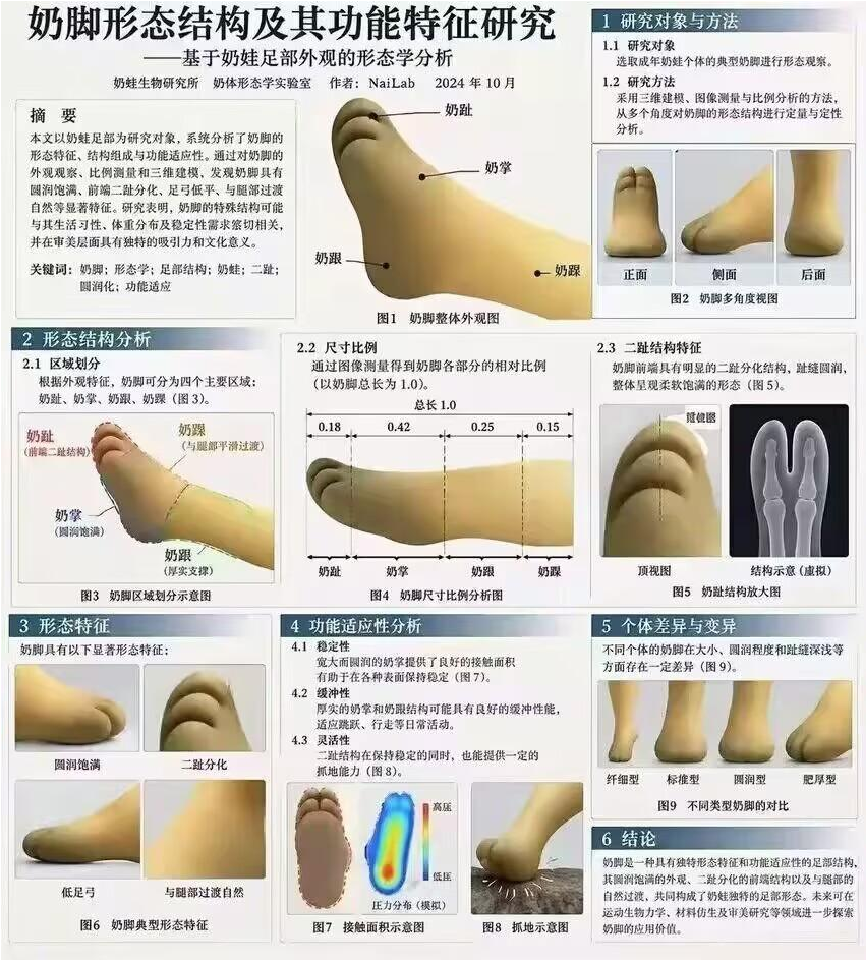
\includegraphics[width=273.19bp,height=0.76\textheight,keepaspectratio]{figures/chapter11/figure11_16.pdf}
  \renewcommand{\thefigure}{11.16}
  \caption{奶蛙户型设计（左）和掌握单片机力量的奶蛙（右）}
  \label{fig:11-16}
\end{figure}


\subsection{九、奶地理学}

“世界就是一个巨大的奶蛙。”这是奶地理学的真谛。~(见\figref{fig:11-17})

% !TEX root = ../../main.tex
\begin{figure}[H]
  \centering
  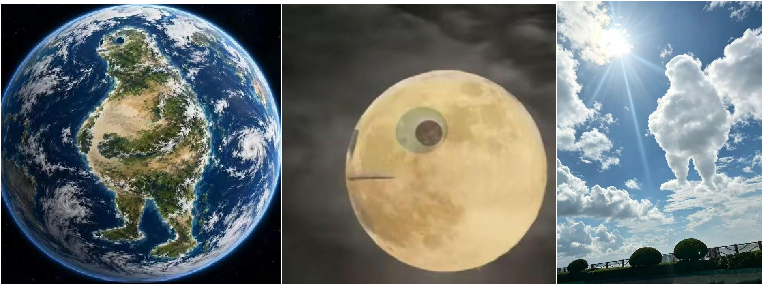
\includegraphics[width=311.13bp,height=0.76\textheight,keepaspectratio]{figures/chapter11/figure11_17.pdf}
  \renewcommand{\thefigure}{11.17}
  \caption{奶地球的古大陆（左）、奶月球（中）、奶云层（右）}
  \label{fig:11-17}
\end{figure}


\clearpage
% Source PDF page 56.
\subsection{十、奶体育运动学}

“你跑不过我你信吗？”这是奶雪峰牢师曾经说过的名言。虽然大家不愿意运动是正常的，但是，在学校和公司我们就练起来\textasciitilde{}~(见\figref{fig:11-18}, \figref{fig:11-19})

% !TEX root = ../../main.tex
\begin{figure}[H]
  \centering
  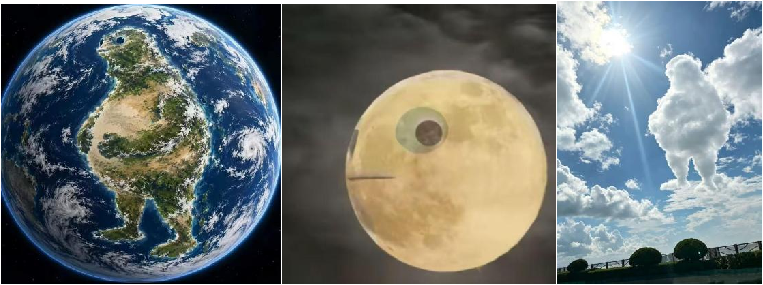
\includegraphics[width=311.13bp,height=0.76\textheight,keepaspectratio]{figures/chapter11/figure11_18.pdf}
  \renewcommand{\thefigure}{11.18}
  \caption{奶地球的古大陆（左）、正在思考要不要引发潮汐的奶月球（中）、奶云层（右）}
  \label{fig:11-18}
\end{figure}


% !TEX root = ../../main.tex
\begin{figure}[H]
  \centering
  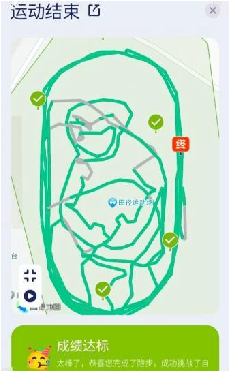
\includegraphics[width=267.17bp,height=0.76\textheight,keepaspectratio]{figures/chapter11/figure11_19.pdf}
  \renewcommand{\thefigure}{11.19}
  \caption{正在打乒乓球的奶蛙（？！赶紧上？！）}
  \label{fig:11-19}
\end{figure}


\subsection{十一、奶考古学}

根本就没有这样的文物！（你只是怕了）~(见\figref{fig:11-20})

% !TEX root = ../../main.tex
\begin{figure}[H]
  \centering
  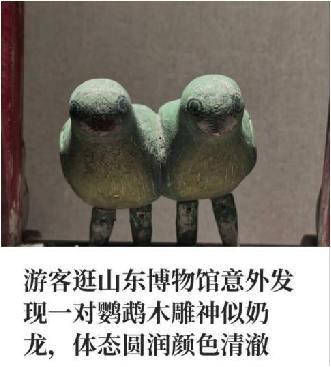
\includegraphics[width=267.17bp,height=0.76\textheight,keepaspectratio]{figures/chapter11/figure11_20.pdf}
  \renewcommand{\thefigure}{11.20}
  \caption{正在打乒乓球的奶蛙（？！赶紧上？！）}
  \label{fig:11-20}
\end{figure}


\clearpage
% Source PDF page 57.
\subsection{十二、奶游戏娱乐学}

在奶国杀里面，奶蛙的强度究竟阴间不阴间？

我们脑杀推测，奶蛙在军八里面的强度绝对不高，但是娱乐性节目效果极强。奶蛙只有三滴血，相当于一个脆皮白板将，但是技能\textbf{【大笑】}可以像病毒一样蔓延开来，把所有人都慢慢变成白板将，就算被打下场也仍然影响着全局。这种特性让奶蛙就算是顶阴局也能有一席之地，只不过选出来不是为了赢，而是为了玩。当所有人的技能都变成\textbf{【大笑】}，胜负根本已经不重要了。这张卡完美契合奶蛙大笑的传染力，设计给到夯。~(见\figref{fig:11-21})

% !TEX root = ../../main.tex
\begin{figure}[H]
  \centering
  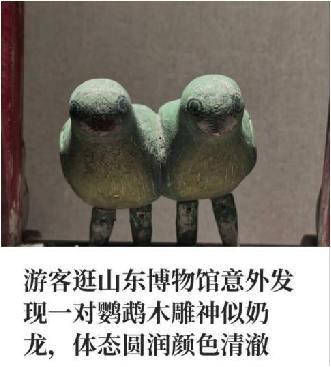
\includegraphics[width=173.74bp,height=0.76\textheight,keepaspectratio]{figures/chapter11/figure11_21.pdf}
  \renewcommand{\thefigure}{11.21}
  \caption{奶国杀中奶蛙的武将牌（作者：阿茶妹妹）}
  \label{fig:11-21}
\end{figure}


\clearpage
% !TEX root = ../main.tex

\clearpage
% Source PDF page 50.
\section{尾声\quad 奶蛙不叛}
\begin{center}
\itshape
\fontsize{13}{24}\selectfont
奶蛙，带着捧腹大笑而来。\par
\vspace{16pt}
没有勾心斗角，没有规矩条框。\\
没有拼死内卷，没有躺平摆烂。\\
没有施加 PUA，没有拉升 BMI。\\
没有卡你 CET，没有让你 EMO。\par
\vspace{16pt}
自由的龙儿是关不住的。\\
所以，\\
发自内心地，\\
无忧无虑地，\\
积极开朗地，\\
随奶蛙，\\
随我，\\
随大家，\\
笑出来吧。\par
\vspace{16pt}
奶蛙不叛，\\
快乐永存。
\end{center}

\begin{flushright}
\small （舍友：你敢自己读一遍吗？）
\end{flushright}


\clearpage
% !TEX root = ../main.tex

\clearpage
% Source PDF page 59.
\section{第一版后记}

好的，本书到此结束\textasciitilde{}

欢迎各高校的奶龙同好会分享本书、使用本书作为社团教材。本书为纯开源乐子书籍，欢迎各位奶家人以本校的奶蛙活动为基础进行教材版本的更新与补充。

鄙人们奶疏学浅，本书关于奶蛙的知识如有错误，请您谅解！

% !TEX root = ../../main.tex
\begin{figure}[H]
  \centering
  \phantomsection
  \addcontentsline{lof}{figure}{\protect\numberline{}后记插图: 我的梦想}
  
\includegraphics[width=249.12bp,height=0.76\textheight,keepaspectratio]{figures/afterword/afterword.pdf}
\end{figure}


下为一些有趣的奶蛙网站：

\begingroup
\small
\noindent \url{https://www.naiwa.world/}\quad 奶蛙档案局\par
\noindent \url{https://github.com/timerring/codex-pet-naiwa}\quad Codex-奶蛙桌宠\par
\noindent \url{https://github.com/Ensurezwwyyds/tokenbaby}\quad Codex-ChatGPT 额度奶蛙倒数器\par
\noindent \url{https://yhsome.github.io/BigNaiWa}\quad 合成大奶蛙\par
\noindent \url{https://66970010-boop.github.io/frog-miner/}\quad 黄金奶工\par
\noindent \url{https://milkyfrog.com/games}\quad 奶蛙游戏大合集（含数十款经典新奇奶蛙游戏！）\par
\endgroup

\begin{flushright}
\bfseries
《捧腹大笑思想与奶龙学概论（第一版）》编写组\par
Tono\_Hanna、Chishoo、Tachibana\_Sherry
\end{flushright}


\clearpage
% !TEX root = ../main.tex

\clearpage
% Source PDF page 60.
\section[参考文献]{参考奶文献}

\begingroup
\small\sffamily
\setlength{\parindent}{0pt}
[1]奶学教研组.奶学导论：从异星幼龙到脑腐图腾——奶龙及其衍生形象通识教材[M/OL].第一版.北京理工大学抽象学出版社,2026.

[2]奶托邦（NAITOPIA）[M/OL].第二卷[出版者不详],2026.

[3]华中科技大学奶蛙群史[M/OL].[出版者不详],2026.

[4]奶龙大学生职业生涯规划[M/OL].[出版者不详],2026.

[5]10.10 蛙龙大战全过程详细经过[M/OL].[出版者不详],2026.
\par
\endgroup

% !TEX root = ../../main.tex
\begin{figure}[H]
  \centering
  \phantomsection
  \addcontentsline{lof}{figure}{\protect\numberline{}参考文献插图}
  
\includegraphics[width=234.94bp,height=0.76\textheight,keepaspectratio]{figures/references/references.pdf}
\end{figure}



\clearpage

\includepdf[pages=1,pagecommand={\thispagestyle{empty}}]{figures/covers/backCover.pdf}
\end{document}
